%% with new filenames distinct from sample-acmlarge.tex.
%% 
%% For distribution of the original source see the terms
%% for copying and modification in the file samples.dtx.
%% 
%% This generated file may be distributed as long as the
%% original source files, as listed above, are part of the
%% same distribution. (The sources need not necessarily be
%% in the same archive or directory.)
%%
%%
%% Commands for TeXCount
%TC:macro \cite [option:text,text]
%TC:macro \citep [option:text,text]
%TC:macro \citet [option:text,text]
%TC:envir table 0 1
%TC:envir table* 0 1
%TC:envir tabular [ignore] word
%TC:envir displaymath 0 word
%TC:envir math 0 word
%TC:envir comment 0 0
%%
%% The first command in your LaTeX source must be the \documentclass
%% command.
%%
%% For submission and review of your manuscript please change the
%% command to \documentclass[manuscript, screen, review]{acmart}.
%%
%% When submitting camera ready or to TAPS, please change the command
%% to \documentclass[sigconf]{acmart} or whichever template is required
%% for your publication.
%%
%%
\documentclass[acmlarge]{acmart}%anonymous

%%
%% \BibTeX command to typeset BibTeX logo in the docs
\AtBeginDocument{%
  \providecommand\BibTeX{{%
    Bib\TeX}}}

%% Rights management information.  This information is sent to you
%% when you complete the rights form.  These commands have SAMPLE
%% values in them; it is your responsibility as an author to replace
%% the commands and values with those provided to you when you
%% complete the rights form.
\setcopyright{cc}
\setcctype{by-nc-sa}
\acmJournal{IMWUT}
\acmYear{2025} \acmVolume{9} \acmNumber{1} \acmArticle{210} \acmMonth{3}
%\acmPrice{0}
\acmDOI{10.1145/3712289}

% \setcopyright{acmlicensed}
% \acmJournal{IMWUT}
% \acmYear{2024} \acmVolume{8} \acmNumber{2} \acmArticle{00} \acmMonth{0}\acmDOI{00.0000/0000000}

%%
%%  Uncomment \acmBooktitle if the title of the proceedings is different
%%  from ``Proceedings of ...''!
%%
%%\acmBooktitle{Woodstock '18: ACM Symposium on Neural Gaze Detection,
%%  June 03--05, 2018, Woodstock, NY}
\acmISBN{978-1-4503-XXXX-X/18/06}


%%
%% Submission ID.
%% Use this when submitting an article to a sponsored event. You'll
%% receive a unique submission ID from the organizers
%% of the event, and this ID should be used as the parameter to this command.
%%\acmSubmissionID{123-A56-BU3}

%%
%% For managing citations, it is recommended to use bibliography
%% files in BibTeX format.
%%
%% You can then either use BibTeX with the ACM-Reference-Format style,
%% or BibLaTeX with the acmnumeric or acmauthoryear sytles, that include
%% support for advanced citation of software artefact from the
%% biblatex-software package, also separately available on CTAN.
%%
%% Look at the sample-*-biblatex.tex files for templates showcasing
%% the biblatex styles.
%%

%%
%% The majority of ACM publications use numbered citations and
%% references.  The command \citestyle{authoryear} switches to the
%% "author year" style.
%%
%% If you are preparing content for an event
%% sponsored by ACM SIGGRAPH, you must use the "author year" style of
%% citations and references.
%% Uncommenting
%% the next command will enable that style.
%%\citestyle{acmauthoryear}

\usepackage{xspace}
\usepackage{enumitem}
\usepackage[capitalise,noabbrev]{cleveref}
\usepackage{tabularx}
%\usepackage{fontspec}
%\newfontfamily{\SymbolaEmoji}{Symbola}
\usepackage{listings}
\usepackage{tcolorbox}
\usepackage{tikz}
\usepackage{longtable}
\usepackage{subcaption}
\usepackage{booktabs}
\usepackage{xcolor}
\usepackage{color, colortbl}

\definecolor{Gray}{gray}{0.9}
\definecolor{LightGray}{gray}{0.6}

\usetikzlibrary{backgrounds}

\newcommand{\dataset}{\textit{DiversityOne}\xspace}
\newcommand{\goto}[1]{\textbf{#1}}

\newcommand{\nilogusers}{782\xspace}
\newcommand{\nsensors}{26\xspace}

\newcommand{\errorcell}[1]{\color{orange}{#1}}
\newcommand{\warningcell}[1]{}%{\color{orange}{#1}}
\newcommand{\goodcell}[1]{\color{green}{#1}}

% for vertical alignment of emoji
\newcommand{\vcenteredinclude}[1]{\begingroup
\setbox0=\hbox{\includegraphics[height=1.5em]{#1}}%
\parbox{\wd0}{\box0}\endgroup}

% Define the tcolorbox style
%\iffalse 
\tcbset{
    mytakeaway/.style={
        colframe=black,           % Border color
        colback=white,            % Background color
        boxrule=0.4pt,            % Border thickness
        fonttitle=\itshape,       % Title font style
        sharp corners,            % No rounded corners
        coltitle=black,           % Title color
        before skip=10pt,         % Space before the box
        after skip=10pt,          % Space after the box
        title={\color{black}},  % Title text and style
        colbacktitle=white,       % Title background color
        coltitle=black,           % Title text color
        attach title to upper,    % Attach title to the top of the box
        boxed title style={
            size=small,           % Title size
            boxrule=0.4pt,        % Title border thickness
            colframe=black        % Title border color
        }
    }
}
%\fi 

\usepackage{soul}
% CHANGE TRACK
% \newcommand{\cancel}[1]{\textcolor{blue}{\st{#1}}}
% \newcommand{\change}[1]{\textcolor{blue}{#1}}
% CAMERA READY: uncomment following lines and comment lines above
\newcommand{\cancel}[1]{}
\newcommand{\change}[1]{#1}


\newcommand{\aau}{Aalborg University\xspace}
\newcommand{\lse}{London School of Economics and Political Science\xspace}
\newcommand{\uc}{Universidad Católica ``Nuestra Señora de la Asunción''\xspace}
\newcommand{\jlu}{Jilin University\xspace}
\newcommand{\ipicyt}{Instituto Potosino de Investigación Científica y Tecnológica\xspace}
\newcommand{\unitn}{University of Trento\xspace}
\newcommand{\amrita}{Amrita Vishwa Vidyapeetham\xspace}
\newcommand{\num}{National University of Mongolia\xspace}

\newcommand{\AAU}{AAU\xspace}
\newcommand{\LSE}{LSE\xspace}
\newcommand{\UC}{UC\xspace}
\newcommand{\JLU}{JLU\xspace}
\newcommand{\IPICYT}{IPICYT\xspace}
\newcommand{\UNITN}{UNITN\xspace}
\newcommand{\AMRITA}{AMRITA\xspace}
\newcommand{\NUM}{NUM\xspace}

% \newcommand{\AAU}{UNI-DEN\xspace}
% \newcommand{\LSE}{UNI-UK\xspace}
% \newcommand{\UC}{UNI-PAR\xspace}
% \newcommand{\JLU}{UNI-CHI\xspace}
% \newcommand{\IPICYT}{UNI-MEX\xspace}
% \newcommand{\UNITN}{UNI-ITA\xspace}
% \newcommand{\AMRITA}{UNI-IND\xspace}
% \newcommand{\NUM}{UNI-MON\xspace}



%%%%%%%%%%%%%%%%%%%%%%%%%%%%%%%%%%%%%%%%%%
%%%%%%%%%%%%%%%%%%%%%%%%%%%%%%%%%%%%%%%%%%

%%
%% end of the preamble, start of the body of the document source.
\begin{document}

%%
%% The "title" command has an optional parameter,
%% allowing the author to define a "short title" to be used in page headers.
%% Pure dataset papers should include the “dataset” keyword in the title
\title[\dataset Dataset]{\textit{DiversityOne}: A Multi-Country Smartphone Sensor Dataset for Everyday Life Behavior Modeling}

%%
%% The "author" command and its associated commands are used to define
%% the authors and their affiliations.
%% Of note is the shared affiliation of the first two authors, and the
%% "authornote" and "authornotemark" commands
%% used to denote shared contribution to the research.


\author{Matteo Busso}
\orcid{0000-0002-3788-0203}
%\affiliation{\institution{University of Trento}\country{Italy}}
\email{matteo.busso@unitn.it}
\authornote{Corresponding author}
%
\author{Andrea Bontempelli}
\orcid{0000-0001-7037-5797}
%\affiliation{\institution{University of Trento}\country{Italy}}
%\email{andrea.bontempelli@unitn.it}
%
\author{Leonardo Javier Malcotti}
\orcid{0009-0000-0589-6393}
\affiliation{\institution{University of Trento}\country{Italy}}
%\email{leonardo.malcotti@studenti.unitn.it}
%
\author{Lakmal Meegahapola}
\orcid{0000-0002-5275-6585}
\affiliation{\institution{ETH Zurich}\country{Switzerland}}
%\email{lakmalbuddikalucky@gmail.com}
%
\author{Peter Kun}
\orcid{0000-0003-0778-7662}
\affiliation{\institution{IT University of Copenhagen}\country{Denmark}}
%\email{peter@peterkun.com}
%
\author{Shyam Diwakar}
\orcid{0000-0003-1546-0184}
%\affiliation{\institution{Amrita Vishwa Vidyapeetham}\country{India}}
%\email{shyam@amrita.edu}
%
\author{Chaitanya Nutakki}
\orcid{0000-0002-5164-2391}
\affiliation{\institution{Amrita Vishwa Vidyapeetham}\country{India}}
%\email{chaithanyakumar@am.amrita.edu }
%
\author{Marcelo Dario Rodas Britez}
\orcid{0000-0002-7607-7587}
\affiliation{\institution{University of Trento \& FBK}\country{Italy}}
%\email{rodas.marcelo@gmail.com}
%
\author{Hao Xu}
\orcid{0000-0001-8474-0767}
%\affiliation{\institution{Jilin University}\country{China}}
%\email{xuhao@jlu.edu.cn}
%
\author{Donglei Song}
\orcid{0000-0001-6737-6932}
\affiliation{\institution{Jilin University}\country{China}}
%\email{songdl17@mails.jlu.edu.cn}
%
\author{Salvador Ruiz Correa}
\orcid{0000-0002-2918-6780}
%\affiliation{\institution{Instituto Potosino de Investigación Científica y Tecnológica}\country{Mexico}}
%\email{salvador.ruiz@ipicyt.edu.mx}
%
\author{Andrea-Rebeca Mendoza-Lara}
\orcid{0000-0003-2301-2891}
\affiliation{\institution{Instituto Potosino de Investigación Científica y Tecnológica}\country{Mexico}}
%\email{anddrea.lara@ipicyt.edu.mx}
%
\author{George Gaskell}
\orcid{0000-0001-6135-9496}
%\affiliation{\institution{London School of Economics and Political Science}\country{UK}}
%\email{g.gaskell@lse.ac.uk}
%
\author{Sally Stares}
\orcid{0000-0003-4697-0347}
%\affiliation{\institution{London School of Economics and Political Science}\country{UK}}
%\email{sally.stares@city.ac.uk}
%
\author{Miriam Bidoglia}
\orcid{0000-0002-1583-6551}
\affiliation{\institution{London School of Economics and Political Science}\country{UK}}
%\email{m.bidoglia@lse.ac.uk}
%
\author{Amarsanaa Ganbold}
\orcid{0000-0003-4335-6608}
%\affiliation{\institution{National University of Mongolia}\country{Mongolia}}
%\email{amarsanaag@num.edu.mn}
%
\author{Altangerel Chagnaa}
\orcid{0000-0003-2331-3045}
\affiliation{\institution{National University of Mongolia}\country{Mongolia}}
%\email{altangerel@num.edu.mn}
%
\author{Luca Cernuzzi}
\orcid{0000-0001-7803-1067}
%\affiliation{\institution{Universidad Católica "Nuestra Señora de la Asunción"}\country{Paraguay}}
%\email{lcernuzz@uc.edu.py}
%
\author{Alethia Hume}
\orcid{0000-0002-1874-1419}
\affiliation{\institution{Universidad Católica "Nuestra Señora de la Asunción"}\country{Paraguay}}
%\email{alethia.hume@uc.edu.py}
%
\author{Ronald Chenu-Abente}
\orcid{0000-0002-1121-0287}
%\affiliation{\institution{University of Trento}\country{Italy}}
%\email{ronaldchenu@gmail.com}
%
\author{Roy Alia Asiku}
\orcid{0009-0004-0369-6151}
%\affiliation{\institution{University of Trento}\country{Italy}}
%\email{royalia.asiku@unitn.it}
%
\author{Ivan Kayongo}
\orcid{0009-0007-4429-7335}
\affiliation{\institution{University of Trento}\country{Italy}}
%\email{ivan.kayongo@unitn.it}
%
\author{Daniel Gatica-Perez}
\orcid{0000-0001-5488-2182}
\affiliation{\institution{Idiap Research Institute \& EPFL}\country{Switzerland}}
%\email{gatica@idiap.ch}
%
\author{Amalia de Götzen}
\orcid{0000-0001-7214-5856}
\affiliation{\institution{Aalborg University}\country{Denmark}}
%\email{ago@create.aau.dk}
%
\author{Ivano Bison}
\orcid{0000-0002-9645-8627}
\affiliation{\institution{University of Trento}\country{Italy}}
%\email{ivano.bison@unitn.it}
%
\author{Fausto Giunchiglia}
\orcid{0000-0002-5903-6150}
\affiliation{\institution{University of Trento}\country{Italy}}
\email{fausto.giunchiglia@unitn.it}




%%
%% By default, the full list of authors will be used in the page
%% headers. Often, this list is too long, and will overlap
%% other information printed in the page headers. This command allows
%% the author to define a more concise list
%% of authors' names for this purpose.

%\renewcommand{\shortauthors}{ANONIMIZED AUTHORS}
\renewcommand{\shortauthors}{Busso et al.}

%%
%% The abstract is a short summary of the work to be presented in the
%% article.

\begin{abstract}
Understanding everyday life behavior \change{of young adults} through personal devices, e.g., smartphones and smartwatches, is key for various applications, from enhancing the user experience in mobile apps to enabling appropriate interventions in digital health apps. Towards this goal, previous studies have relied on datasets combining passive sensor data with human-provided annotations or self-reports. %The ultimate goal was to develop machine learning models that infer various aspects of everyday life, including mood, activities, social context, and eating habits. 
However, many existing datasets are limited in scope, often focusing on specific countries primarily in the Global North, involving a small number of participants, or using a limited range of pre-processed sensors. These limitations restrict the ability to capture cross-country variations of human behavior, including the possibility of studying model generalization, and robustness. To address this gap, we introduce \textit{DiversityOne}, a dataset which spans eight countries (China, Denmark, India, Italy, Mexico, Mongolia, Paraguay, and the United Kingdom) and includes data from \nilogusers college students over four weeks. DiversityOne contains data from \change{\nsensors smartphone sensor modalities} and 350K+ self-reports. As of today, it is one of the largest and most diverse publicly available datasets, while featuring extensive demographic and psychosocial survey data. DiversityOne opens the possibility of studying important research problems in ubiquitous computing, particularly in domain adaptation and generalization across countries, all research areas so far largely underexplored because of the lack of adequate datasets. 

\vspace{1em}
\tikzstyle{background rectangle}=[thin,draw=black]
\begin{center}
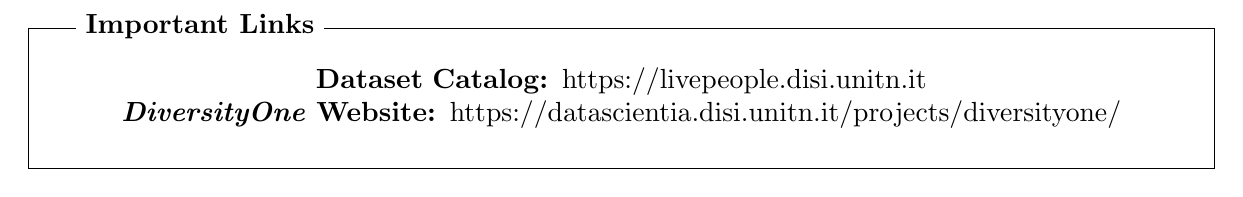
\begin{tikzpicture}[show background rectangle]
\node[align=center, text width=40em, inner sep=1em]{
%Not included for now due to double-blind review
\textbf{Dataset Catalog:} \url{https://livepeople.disi.unitn.it} \\
\textbf{\dataset Website:} \url{https://datascientia.disi.unitn.it/projects/diversityone/}
};
\node[xshift=3ex, yshift=-0.7ex, overlay, fill=white, draw=white, above 
right] at (current bounding box.north west) {
\textbf{Important Links}
};
\end{tikzpicture}
\end{center}

\end{abstract}

%%
%% The code below is generated by the tool at http://dl.acm.org/ccs.cfm.
%% Please copy and paste the code instead of the example below.
%%
\begin{CCSXML}
<ccs2012>
   <concept>
       <concept_id>10003120.10003138</concept_id>
       <concept_desc>Human-centered computing~Ubiquitous and mobile computing</concept_desc>
       <concept_significance>500</concept_significance>
       </concept>
   <concept>
       <concept_id>10003120.10003138.10011767</concept_id>
       <concept_desc>Human-centered computing~Empirical studies in ubiquitous and mobile computing</concept_desc>
       <concept_significance>300</concept_significance>
       </concept>
   <concept>
       <concept_id>10003120.10003138.10003141.10010895</concept_id>
       <concept_desc>Human-centered computing~Smartphones</concept_desc>
       <concept_significance>300</concept_significance>
       </concept>
   <concept>
       <concept_id>10003120.10003138.10003139.10010905</concept_id>
       <concept_desc>Human-centered computing~Mobile computing</concept_desc>
       <concept_significance>300</concept_significance>
       </concept>
 </ccs2012>
\end{CCSXML}

\ccsdesc[500]{Human-centered computing~Ubiquitous and mobile computing}
\ccsdesc[300]{Human-centered computing~Empirical studies in ubiquitous and mobile computing}
\ccsdesc[300]{Human-centered computing~Smartphones}
\ccsdesc[300]{Human-centered computing~Mobile computing}

%%
%% Keywords. The author(s) should pick words that accurately describe
%% the work being presented. Separate the keywords with commas.
\keywords{datasets, diversity, social practices, mobile sensing, smartphone sensing, wellbeing, health, generalization}

\received{20 February 2007}
\received[revised]{12 March 2009}
\received[accepted]{5 June 2009}

%%
%% This command processes the author and affiliation and title
%% information and builds the first part of the formatted document.
\maketitle

\section{Introduction} \label{sec:intro}
Human behavior, routines, habits, and social practices are deeply interwoven with the events, places, interactions, and technologies that compose our everyday lives. Each of these elements contributes to larger behavioral patterns influenced by our continuous engagement with pervasive devices. Our emotional experiences fluctuate daily, shaped by factors such as sleep quality \cite{khalid2024sleepnet}, which, in turn, impact our physical activity, forming both recurring weekly patterns \cite{tseng2016assessing} and longer-term habits \cite{harari202019}. Everyday actions, such as eating and drinking, also have significant effects on our health \cite{biel2018bites, santani2018drinksense}, with additional factors like interactions with technology playing important roles in everyday life  \cite{das2019multisensor}.


Smartphones, as prevalent devices in daily life, influence our behavior, often in nuanced ways that can be both positive \cite{lin2021revisiting} and negative \cite{2017-SOCINFO}. Their use is linked to our internal states \cite{elhai2018depression, buda2021outliers}, and understanding how people engage with their smartphones could provide valuable insights into human behavior. Prior research has shown that smartphone sensors can infer a range of behavioral aspects in young adults, including mood \cite{servia2017mobile, meegahapola2023generalization}, depression \cite{xu2023globem}, activities \cite{haresamudram2021contrastive, assi2023complex}, social context \cite{mader2024learning, hernandez2024proximity}, and eating or drinking episodes \cite{bae2017detecting, santani2018drinksense, thomaz2016automatic, biel2018bites}. This makes smartphone sensor data valuable for improving app design, supporting user well-being, and creating more effective interventions. However, there are profound variations in daily behaviors across different cultural and geographic backgrounds \cite{foner2020introduction}\footnote{\change{We operationalize the concept of culture through the theory of social practices outlined in \cref{subsubsec:soa-socio}. This concept recognizes that cultures are complex and multidimensional, often coexisting or overlapping within the same geographic areas \cite{yuval2004gender}. Additionally, it acknowledges that certain regularities emerge from specific socio-cultural contexts or from the communities of practice that develop locally. The use of terms like ``country,” ``culture,” and ``geographic region” throughout the paper reflects this distinction.}}. Ignoring these variations has often hindered model generalization \cite{meegahapola2023generalization, khwaja2019modeling}, limiting the effectiveness of behavior inference models when applied in diverse real-world settings.


Despite the richness of smartphone sensor data, a critical challenge persists: the lack of datasets that capture behavioral diversity across different cultural and geographic contexts. Existing datasets and research often draw from specific populations typically in the Global North \cite{khwaja2019modeling, meegahapola2023generalization}, and may not fully account for the cultural, environmental, and social norms that shape daily routines and smartphone usage patterns in other regions \cite{phan2022mobile}. This limits the development of machine learning models capable of generalizing across different populations. For instance, eating habits \cite{tobin2018dinner}, sleep routines \cite{stacker2023sleep, cheung2021considering}, and social interactions \cite{gsir2014social, parady2021comparative} vary widely between countries, affecting how individuals interact with their smartphones and how other daily life aspects are inferred from sensor data \cite{lopez2017self, phan2022mobile}. Consequently, models trained on data from one country or region may perform poorly when applied to another. This underscores a fundamental challenge in generalizing machine learning models to real-world applications \cite{meegahapola2023generalization, assi2023complex}. Addressing this challenge requires comprehensive datasets that not only capture a variety of sensor data but also integrate cultural, social, and geographical diversity. Such datasets would enable researchers to study behavioral differences and similarities across populations, to test model robustness in diverse contexts beyond typical experimental settings\change{, and to investigate how to combine model generalization and adaptation to local data to capture local and individual behaviors.} 

The \dataset dataset, developed as part of the large-scale European project \textit{``WeNet - The Internet of US''}\footnote{\url{https://doi.org/10.3030/823783}.} \cite{2025WenetPaper},
%\footnote{Details to be disclosed post-double-blind review},
provides rich, cross-country data for studying everyday life behavior through smartphone sensors and self-reports. \dataset spans data from college students in eight countries: 
{China} (\jlu, \textbf{\JLU}),
{Denmark} (\aau, \textbf{\AAU}), 
{India} (\amrita, \textbf{\AMRITA}), 
{Italy} (\unitn, \textbf{\UNITN}), 
{Mexico} (\ipicyt, \textbf{\IPICYT}), 
{Mongolia} (\num, \textbf{\NUM}), 
{Paraguay} (\uc, \textbf{\UC}), and 
the {United Kingdom} (\lse, \textbf{\LSE}). 
The study involved more than 18,000 students, of which \nilogusers agreed to participate in an intensive longitudinal survey of four weeks. Based on the innovative \texttt{iLog app}~\cite{2014-PERCOM}, adopted for the data collection, \dataset includes raw data from \nsensors smartphone sensors, such as accelerometers, gyroscopes, and GPS, as well as derived information like notification interactions, app usage, activities, and step counts, during these four weeks. These data streams are organized into six category bundles (connectivity, environment, motion, position, app usage, and device usage), allowing modular downloads for ease of use. Additionally, participants provided multiple in-situ self-reports each day, through time diaries, detailing their activities, locations, social contexts, and moods, together with daily reports on sleep quality and daily expectations. This combination of self-reported data and sensor data provides a comprehensive view of behavior, making \dataset a valuable resource for studying the impact of smartphone technology across various contexts in both the Global North and the Global South \cite{biel2018bites, khalid2024sleepnet, qin2019cross, grammenos2018you}. \change{Additionally, DiversityOne enables more computational social science-oriented studies focused on human behavior (see, e.g., \cite{2017-SOCINFO, zhang2021putting, bontempelli2020learning}).}

The \dataset dataset supports the development of machine learning models capable of inferring user behaviors, with potential applications in domain generalization, domain adaptation\change{, transfer learning}, and self-supervised learning. It is a valuable research resource in ubiquitous computing, human-computer interaction, and machine learning, offering a broader scale than previously available datasets. Furthermore, \dataset adheres to the European General Data Protection Regulation (GDPR) \cite{GDPR2016}, with ethical approvals from all participating institutions. The study design and data collection processes were developed by an interdisciplinary team of computer scientists, social scientists, interaction designers, ethicists, and legal experts to meet the highest standards. This extensive dataset has been used in a few initial publications by different authors, showing its various uses \cite{meegahapola2023generalization,  kammoun2023understanding, assi2023complex,meegahapola2024m3bat, mader2024learning,girardini2023adaptation,mercado2023social}, and demonstrating its potential for reuse in studies aiming to understand behaviors across countries through smartphone sensing. The paper describes three contributions:

\begin{itemize}[wide, labelwidth=!, labelindent=0pt]

\item[\textbf{Contribution 1:}] We publicly release \dataset, one of the largest and most geographically diverse datasets combining questionnaires from 18K+ participants and passive smartphone sensor data and self-reports from \nilogusers participants across eight countries, covering both the Global North and the Global South. The dataset includes raw sensor data from \nsensors modalities, providing researchers with a flexible resource for analyzing and developing machine learning models across multiple domains, such as behavior recognition, cross-cultural studies, and multimodal time-series modeling. This dataset facilitates explorations of topics like model generalization and domain adaptation across countries, with detailed self-reports on demographic and psychosocial variables, adding depth for nuanced, multifaceted analyses that can be conducted independently or integrated with sensor data.

\item[\textbf{Contribution 2:}] We provide an in-depth description of the study design and data collection, which was tailored to enable effective data gathering across multiple countries, each with unique languages, privacy regulations, and cultural contexts (Section~\ref{sec:method}). To manage the diversity and sensitivity of the collected data, the dataset was consolidated under rigorous privacy and ethical standards, hosted in a GDPR-compliant secure environment, and respecting the ownership rights of all contributors.


\item[\textbf{Contribution 3:}] We synthesize key insights, lessons learned, and recommendations derived from some initial studies leveraging \dataset, highlighting unique opportunities for further studies in smartphone sensing, behavioral modeling, and machine learning. We provide the insights under two broader themes---Lessons learned from (i) study design and cross-country data collection (\cref{subsec:lessons_design}) and (ii) multi-country sensor data analysis (\cref{subsec:lessons_analysis}). Our 12 recommendations, which we see as actionable, aim to provide ideas for future research, enhancing the adaptability and accuracy of smartphone-based behavioral studies in diverse global contexts.

\end{itemize}


The remainder of the paper is organized as follows: \cref{sec:relatedworks} provides background and context for the methodology used to create \dataset, reviewing existing datasets for modeling everyday behaviors through smartphone sensors alongside various forms of ground truth. \cref{sec:method} details the methodology and protocol adopted to collect diverse, cross-country data, with specific attention to variations in cultural contexts of student's daily routines and data privacy regulations. \cref{sec:validation} presents key results to validate the data collection approach and the dataset's quality. \cref{sec:availability} outlines the resources available for accessing and using the dataset, highlighting compliance with privacy and copyright standards. \cref{sec:discussion} explores potential use cases for the dataset, provides insights and recommendations, emphasizing its value in studying behavioral patterns across different regions and advancing machine learning applications. Lastly, \cref{sec:conclusion} summarizes the paper’s contributions and impacts.

\section{Background and Related Work}\label{sec:relatedworks}
\subsection{Smartphone Sensing for Behavior Modeling}

Smartphone sensing data is widely used to train machine learning models to infer user behaviors in real-world environments \cite{meegahapola2020smartphone}. Developing these models involves continuously collecting data from sensors like accelerometers, gyroscopes, GPS, Bluetooth, and app usage logs to create labeled datasets. These datasets serve as ground truth for various behaviors, including daily activities, social interactions, mental states, sleep, and dietary habits \cite{meegahapola2020smartphone}. These labeled datasets fuel machine learning models, from classic approaches (e.g., random forest, decision tree, support vector machines) to deep learning techniques, enabling the detection of behavioral patterns and predictions on new, unseen data. Once trained, these models are deployed in-the-wild, running on users' smartphones to provide real-time insights into daily routines, mental well-being, and contextual changes, all without requiring active input from the user. Traditionally, such models have relied heavily on continuous sensing modalities—such as movement patterns and physical proximity—to infer user behavior. More recently, however, interaction sensing modalities (e.g., app usage, typing events, and notification interactions) have gained significance, providing rich insights into users’ engagement patterns and internal states.

\subsection{Continuous and Interaction Sensing Modalities} Smartphone sensors can be broadly classified into two types \cite{meegahapola2020smartphone}: continuous sensing and interaction sensing, both essential for understanding nuances of everyday life.

Continuous sensing involves passive data collection without direct user interaction. For instance, accelerometers and gyroscopes detect movement patterns (e.g., walking, running, or inactivity) that offer insights into physical activity levels and types, relevant for understanding behavioral patterns, energy expenditure, and emotional states, such as depression or anxiety indicated by prolonged inactivity or erratic movements~\cite{elhai2018depression, canzian2015trajectories}. Step count, derived from inertial sensors, further enhances activity monitoring, revealing daily routines and physical well-being. Additionally, proximity sensors and Bluetooth signals can indicate social contexts by identifying close proximity to others, which helps assess social isolation or engagement~\cite{meegahapola2020smartphone, lane2010survey}. GPS and WiFi data are indispensable for determining semantic locations, enabling insights into whether users are at home, at work, or engaged in recreational activities—each of which correlates with mental states or other behavioral patterns~\cite{santani2018drinksense, meegahapola2023generalization, servia2017mobile}.

Interaction sensing captures smartphone user engagement, providing insights into attention, productivity, and emotional states. App usage, for example, can infer attention spans, productivity, and even stress levels, as excessive or reduced engagement with certain apps may be linked to anxiety or depressive symptoms~\cite{guracho2023smartphone}. Studies have shown that interactions with social media, in particular, are tied to mental well-being~\cite{buda2021outliers}. Similarly, frequent typing events, rapid touch interactions, or ignoring notifications can signal heightened stress or distraction \cite{vahedi2018association}. Notifications, app-opening frequencies, and related metrics also provide important context for attention spans and can identify potentially compulsive behaviors, such as frequent app-checking, which may indicate underlying mental health concerns \cite{meegahapola2020smartphone, carlo2019numbers}.

Combining continuous and interaction sensing modalities offers a comprehensive view of behavior, allowing machine learning models to capture nuanced and expressive aspects with a high level of detail. Currently available public smartphone sensing datasets, however, often lack this level of depth and diversity in sensing modalities, limiting the ability to fully understand human behavior at scale. Even if many modalities are present, most publicly available datasets only offer pre-processed versions of data, limiting the use of such datasets for diverse purposes. Therefore, there is an unmet need for raw smartphone sensor datasets that integrate continuous and interaction sensing modalities, offering richer insights into behavioral patterns. 

\subsection{Effect of Country Diversity on Sensing and Self-reported Ground Truth}

Together, continuous and interaction-sensing modalities build a holistic picture of user behavior, capturing both passive and longitudinal patterns and immediate interactions that correlate with mental and emotional states. However, sensor data and self-reported behaviors used as ground truth for training machine learning models can vary significantly across countries, influenced by cultural, social, and environmental differences \cite{phan2022mobile}.

For example, sensor data like accelerometer readings or step counts may reflect distinct physical activity patterns based on country-specific factors, such as urban infrastructure, transportation habits, and climate \cite{ICLEI_UrbanTransport, ZeroHourClimate_UrbanPlanning, EPA_ClimateTransportation}. In countries where walking or cycling is common, step counts may show higher physical activity levels, while regions reliant on driving will have lower activity levels. Similarly, proximity sensor and Bluetooth data capture different social interaction patterns, reflecting cultural norms around personal space, social gatherings, and work environments \cite{ozella2021using, janssen2024tracking, sekara2014strength, hernandez2024proximity}. In collectivist cultures, for instance, users may exhibit more frequent close proximity with others, while individualistic cultures may show more solitary sensor readings \cite{trumbull2001bridging, triandis2001individualism}. Cultural attitudes towards technology could also shape app usage and notification interactions \cite{bombardi2017exploring}. Social media may dominate app engagement in some countries, whereas others might have more work-focused or communication-restricted technology use \cite{poushter2018social, cheng2021prevalence}. Beyond sensing modalities, the way behaviors are reported as ground truth---such as moods, stress, context, or activity types---varies culturally \cite{mesquita1992cultural, meegahapola2023generalization, sebe2005multimodal}. Cultural norms can influence self-reported stress or mood, leading to different labels for similar sensor data patterns across countries \cite{schmidt2019wearable, mesquita1992cultural, meegahapola2024m3bat}. In machine learning terms, such cross-country variations introduce challenges related to data covariate shift and label shift, both of which complicate generalization \cite{bickel2009discriminative, koh2021wilds}.

Despite these evident variations, most prior studies overlook country-level differences, relying on homogeneous datasets from specific regions, often within the Global North \cite{meegahapola2020smartphone, phan2022mobile}. This oversight leads to models that struggle to generalize effectively to diverse populations and cultural contexts. In some instances, even though cross-country data were available, analysis has not focused on country differences \cite{servia2017mobile}. Without datasets that capture country-specific data and behavioral patterns, machine learning models are likely to produce incorrect inferences when applied outside the regions in which they were trained. To improve model robustness, globally diverse datasets are essential for exploring behavioral differences across populations, allowing models to account for the variations in behaviors and sensor data across countries and cultures. Addressing this gap is one of the main objectives of the \dataset dataset.

Furthermore, collecting large-scale, passive smartphone sensing data with accurate labels is challenging due to significant costs, time, and effort, especially when collecting data from diverse international participants \cite{yfantidou2023beyond}. Datasets in this field typically involve fewer than 100 participants (see Table~\ref{tab:relatedwork}) since managing continuous data streams, conducting longitudinal data collection, and providing accurate behavioral labels make scaling these studies complex. Scaling up to engage hundreds of participants requires intensive recruitment, sustained user engagement, and technical infrastructure to handle continuous sensor data collection over extended periods. This is partly why the field of ubiquitous computing (ubicomp) lags behind fields like computer vision or natural language processing, where collecting millions of labeled images, videos, or text is relatively more straightforward and cost-effective, enabling faster progress. However, data collection across countries presents additional challenges, as cultural, behavioral, and infrastructure differences influence how people use smartphones, complicating the labeling process. Unlike images, videos, or text, which can be labeled through standardized methods or crowdsourcing, passive sensing data requires detailed, context-specific labeling of behaviors like mood, activity, and social interaction, often relying on time-consuming self-reports. Cross-country collection further complicates matters with logistical issues such as language differences, varying ethical standards, and compliance with different data privacy laws. These challenges make large-scale, diverse data collection costly and time-intensive. The \dataset dataset’s achievement in collecting data from \nilogusers participants demonstrates the commitment and resources required to overcome these hurdles.

\change{\subsection{Sociological Theory and Approaches to Study Design} 
}\subsubsection{Cultural Diversity as Social Practices} \label{subsubsec:soa-socio}
\change{The concept of culture has been extensively examined in social sciences. Previously, culture was viewed as a cohesive framework that influenced attitudes and practices through socialization \cite{swidler1986culture}. However, recent studies suggest that culture is fragmented and diverse among social groups \cite{lizardo2016dual}. This shift in perspective sees culture as complex structures of quasi-rules that individuals can use strategically \cite{bourdieu1990logic, sewell1992theory} and highlights the need to analyze relationships among various cultural influences, linking them to distinct phenomena and calling for a more nuanced psychological understanding \cite{cerulo2010mining}. }

The study design of the \dataset dataset focuses on a particular definition of culture, deriving from the social practice theory \cite{wittgenstein1953philosophical,goffman1975asylums,giddens1979central,giddens1984society,bourdieu1977outline,bourdieu1990logic,Dreyfus1991world,schatzki2001practice,reckwitz2002toward}. This theory frames human behavior as composed of daily practices that produce societal outcomes and influence individual skills and mindsets, contributing to social structure and culture. According to \citet{shove2012dynamics}, social practices consist of three key components:

\begin{itemize}
\item \textbf{Material}: The physical objects or resources, such as a car or a membership, that enable the execution of a particular practice.
\item \textbf{Competence}: The knowledge, skills, and abilities that make a certain practice possible.
\item \textbf{Meaning}: The cultural and symbolic elements that give significance to social practices, motivating individuals to perform them in alignment with societal norms.
\end{itemize}
\noindent
For instance, environmental consciousness may motivate individuals to choose public transportation, aligning with behaviors like cycling, waste sorting, or adopting a vegetarian lifestyle. These motivations, shaped by material access (such as bike availability or recycling facilities), personal competence, and meaningful commitment to sustainability, collectively define behaviors that, when widely adopted within a community, become recognized social practices \cite{shove2005consumers,ropke2009theories}. 

\change{Thus, there is a distinction between the practitioner (individual) and the social practice (community). While interconnected, social practices exist independently and are established at the social level. Indeed, \citet{ropke2009theories} noted that practices consist of recognizable, interconnected elements that individuals reproduce, with new members being constantly recruited. In this sense, individuals are ``carriers of practices'' recruited based on their backgrounds, not merely choosing practices by utility \cite{reckwitz2002toward}, and the distribution of practices often reflects social inequality, with varying cultural perceptions of what constitutes ethical practice. Participation in a practice leaves lasting effects, such as knowledge and skills, which facilitate future involvement in that practice in a path-dependent process~\cite{ropke2009theories}. Finally, diversity is socially recognized, and practices are inherently social, resembling one another across different contexts \cite{reckwitz2002toward}. In other words, social practices exhibit regularity - models of how certain daily practices are typically and habitually performed in (a considerable part) of a society \cite{holtz2014generating}.}

\change{This perspective enhances our understanding of human behavior in real-world environments, where the activities recorded by sensors may be limited in terms of quantity, quality, and context representation. Identifying whether an individual belongs to a community of practice and their ``career'' within it enables the inference of important characteristics, such as the nature of their activities—distinguishing, for example, between an athlete's training session or recreational activity—the tools utilized, such as appropriate clothing and supportive technologies, and the likelihood of recurring behavioral patterns over time. This understanding is particularly valuable in situations where data may be limited or less accurate.}

\change{Furthermore, gaining insight into the context in which these practices occur allows for culturally informed comparisons. This encompasses both the individual perspective, which considers the factors that may facilitate or impede engagement in a practice or access to a community, and the social perspective, which examines how the reference community typically interacts with that practice.}

\change{\subsubsection{Capturing Social Practices}} \label{subsubsec:soa-meth}
Researchers utilize various methodologies to effectively capture behaviors and lifestyles over time. In European countries, for example, the Harmonized European Time Use Surveys (HETUS) measure time spent on various activities. At the same time, the Experience Sampling Methodology (ESM) focuses on the interoceptive, or internal, aspects of behavior \cite{csikszentmihalyi2014validity, myin2022esm}. Time-use diaries, commonly used in HETUS, are intensive longitudinal surveys where participants self-report activity sequences over a day, detailing the frequency and duration of their actions to reveal intricate social patterns. Participants typically complete these diaries at regular intervals, tracking each activity, which enables a detailed, objective view of daily routines and interactions \cite{sorokin1939time}. In contrast, ESM prompts participants to report their thoughts and behaviors over days or even months, detailing their personal points of view on their daily experiences. A comprehensive review by \citet{van2017experience} highlights the strengths of ESM in capturing these aspects.

\change{Our approach combines these two perspectives, namely time-use diaries and ESM with smartphone sensor data. For every sensor pattern that indicates an action or habit—such as accelerometer data, Movement Activity Labels, or GPS positions—researchers can reconstruct the individual's social and personal context. 
A study review explores this combination of continuous sensing and interaction sensing with self-report data for the well-being of young adults~\cite{meegahapola2020smartphone}.
Here, self-report data can serve as ground truth events. Conversely, in scenarios like interactive classification in the wild \cite{bontempelli2020learning}, algorithms such as skeptical learning can use sensor information to validate user annotation. Furthermore, this approach enables the researcher to observe human behavior from the individual point of view within the community of practice, specifically her understanding and interpretation of the context in which the activity occurs (see, e.g., \cite{zhang2021putting}).} 


\subsection{Currently Available Public Smartphone Sensing Datasets}

\begin{table}[btp]
\caption{\label{tab:relatedwork} Public available datasets for activity and context recognition in the wild. Duration is expressed in days. The number of pilot sites indicates whether the countries are in the Global North (N) and/or Global South (S). (+) Sensors are divided between smartphones and (+) other devices. No '+' means only smartphone sensors. (*) The GLOBEM data collection was done during a semester for 10 weeks each year, for 4 different years.}
\begin{tabularx}{\textwidth}{lrrcXr}
\toprule
\textbf{Datasets}%
& \multicolumn{3}{c}{\textbf{Coverage}}%
& \multicolumn{2}{c}{\textbf{Purpose}}\\  
\cmidrule(rl){2-4}\cmidrule(rl){5-6}
 & \multicolumn{1}{c}{\textbf{Sample}}         & \multicolumn{1}{c}{\textbf{Days}} & \multicolumn{1}{c}{\textbf{Sites}} & \multicolumn{1}{c}{\textbf{Self-reports}}                          & \multicolumn{1}{c}{\textbf{Sensors}}   \\
\midrule
MDC (2013)   \cite{laurila2013}               & 185                      & 365                      & 1 N                 & Location   
                                        & 12+14                     \\
StudentLife  (2014)  \cite{wang2014studentlife}          & 48                      & 70                      & 1 N                 & Sleep-related                                 & 10                    \\
%MobiAct   (2016) \cite{vavoulas2016mobiact}              & 57                      & Trials                  & 1                 & .                                             & 3                     \\
ExtraSensory  (2017)  \cite{vaizman2017recognizing}      & 60                      & 7                       & 1 N                & Activity                                      & 8+2                 \\
Real-life HAR  (2020)  \cite{gonzalez2020}               & 19                      & 28                      & 1 N                &  .                                            & 4                     \\
ContextLabeler  (2021)  \cite{campana2021contextlabeler} & 3                       & 14                      & 1 N                 & Activity                                      & 18                    \\
Qwantify  (2022)   \cite{wilson2022qwantify}          & 242                     & 7   & 1 N                & Desire, emotion,    well-being                & . \\
LifeSnaps  (2022) \cite{yfantidou2022lifesnaps}           & 71                      & 120 & 4 N & Location, Mood, Step Goal & 0+23 \\
ETRI  (2022) \cite{chung2022real}                         & 22                      & 28                      & 1 N               & Activity, Location,   Relation, Mood          & 10+4                \\
SmartUnitn2  (2018)  \cite{li2022representing}           & 158                     & 28                      & 1 N               & Activity, Location,   Relation, Mood          & 28                    \\
LAUREATE   (2023) \cite{laporte2023laureate}             & 42                      & 91                      & 1 N                 & Activities, Health                            & 0+6                   \\
GLOBEM  (2023) \cite{xu2023globem}                        & 534                     & 280*                     & 4 N              & Standard scales (personality, physical, mental and social well-being)                             & $\sim$10              \\
EgoADL  (2024)  \cite{sun2024multimodal}                 & 30                      & 5                       & 1 N                & Automated labels                              & 4+2                   \\


 & & & & & \\
\textbf{\dataset}                                               & \textbf{\nilogusers}            & \textbf{28}             & \textbf{8 (3N,5S)}        & \textbf{Activity, Location,   Relation, Mood} & \textbf{26}   \\        
\bottomrule
\end{tabularx}
\end{table}

Several datasets that leverage smartphone and smartwatch sensors for activity and context recognition have been developed across various research fields. \cref{tab:relatedwork} compares key publicly available datasets, highlighting their sample size, duration, data collection sites, self-reported questionnaires or annotations via intensive longitudinal survey, and number of sensors used, both collected via smartphone and other devices. While these datasets contribute valuable insights, most are constrained by small sample sizes and short data collection durations, which limit their ability to capture daily routines and behavioral patterns. For instance, although datasets like MDC~\cite{laurila2013}, StudentLife~\cite{wang2014studentlife}, and Real-life HAR~\cite{gonzalez2020} extend beyond short-term studies, they still lack the diversity required to observe routine behaviors that often necessitate more extended observation periods and cross-country differences.


Datasets that focus solely on continuous sensor data, such as Real-life HAR \cite{gonzalez2020}, are limited in capturing the complexity of human activities because they do not include annotations reflecting users' experiences or contexts. Moreover, a growing trend involves using experience sampling methodologies (ESM), where users frequently self-report their experiences, to capture behaviors and contextual nuances. Datasets like the Qwantify app~\cite{wilson2022qwantify} provide valuable insights into emotions, desires, and well-being. Still, sensor data in these collections often remain secondary, serving mainly as context rather than central to the analysis. Hence, \cancel{we believe it is fair to say that}the most valuable datasets combine sensor data with self-reports about the collected data. Such datasets can be further divided into those with in-situ (reports provided about the current moment) and retrospective (reports provided about past periods or days) self-reports~\cite{meegahapola2020smartphone}. A notable example of retrospective self-reporting is the work of \citet{krumm2013placer}, which uses time diaries (i.e., similar to the HETUS approach described in \cref{subsubsec:soa-meth}) for labeling. However, the lack of direct user interaction during labeling can lead to inaccuracies and contextual inconsistencies. In contrast, datasets like StudentLife~\cite{wang2014studentlife}, ExtraSensory~\cite{vaizman2017recognizing}, and ContextLabeler~\cite{campana2021contextlabeler} rely on in-situ self-reports from users. Still, they are often limited to specific activities and do not adhere to a standardized reference, which introduces social and cognitive biases.

GLOBEM \cite{xu2023globem} presents a large-scale dataset that enables cross-dataset generalization analysis, which is particularly valuable for examining behavioral patterns across different periods and university environments. Its longitudinal nature, spanning over \change{four years (ten weeks of data collection each year)}, allows researchers to assess how models perform across diverse academic settings over time. However, the dataset predominantly focuses on the USA, limiting its applicability for cross-country studies. Hence, while GLOBEM provides essential insights, its geographic concentration contrasts with the more globally diverse scope of \dataset, which includes participants from eight countries across the global north and south, offering a broader foundation for generalization and cross-country behavior modeling. Moreover, \dataset provides more fine-grained and raw sensor data and frequent in-situ self-reports, giving researchers much flexibility and depth in their analysis. 

Among existing datasets, LifeSnaps \cite{yfantidou2022lifesnaps} is the most comparable to \dataset in terms of countries of data collection. However, despite the richness, the dataset falls short in crucial areas such as sample size, diversity of data collection countries, and breadth of sensor coverage. LifeSnaps focuses primarily on four European countries and only has a sample size of 71 participants, whereas \dataset spans both the global north and south, including a broader cultural and geographic range, with \nilogusers participants. This comprehensive scope makes \dataset a unique resource for understanding everyday life behavior across diverse countries, surpassing other available datasets in terms of depth and scale.


\subsection{The \dataset Dataset}
\change{Our dataset aims at making a valuable contribution by differing significantly from previous works in several key aspects, as outlined below. First, as described in \cref{subsubsec:soa-meth}, our dataset methodology follows best practices from earlier studies by measuring behaviors and psychosocial traits using standardized and validated methods. We propose a combination of self-reported annotations and sensor data from smartphones. This integration enables a nuanced understanding of social practices, considering routine behaviors alongside contextual data about both physical actions and mental states. While many current datasets aim to capture such elements, few achieve the same depth of blending multiple methodologies with sensor data. This multifaceted approach allows for a more accurate, holistic view of human behavior, providing fine-grained labels essential for training robust machine learning models that reflect the complexity of everyday life. Second, to the best of our knowledge, there are currently no publicly available smartphone datasets specifically tailored to examining social practices (see \cref{subsubsec:soa-socio}). This innovative framework allows researchers to enrich their understanding of individuals by situating them within a broader community of profiles that share similar competencies, materials, and meanings. For instance, it distinguishes between those engaged in professional activities and those pursuing recreational interests, highlighting each group's distinct personalities and values. This nuanced approach encourages researchers to explore the diversity of daily activities in a way that emphasizes the cultural context of behaviors, thereby creating a more comprehensive understanding of how social practices shape individual actions and interactions.}

\change{Finally, our sample size and the breadth of data collected internationally, with a particular emphasis on regions in the global south —underrepresented in prior research— is rather unique. In addition to our theoretical and methodological approach, these characteristics enable a more comprehensive exploration of human behavior, shedding light on the diversity among people and their similarities. In summary, by integrating diverse cultural and socio-demographic factors, \dataset facilitates a deeper exploration of behavior modeling, personalization, and cross-cultural adaptation at a more nuanced level. Moreover, incorporating these factors fosters cross-cultural and multidisciplinary analysis of human behavior rather than promoting it solely as a machine learning benchmark dataset~\cite{orr2024ai,raji2021ai}.}


\section{Methodology}\label{sec:method}
\section{Methods}\label{sec:methods}

In this section we discuss several methods that have an impact on the overall performance of a MINLP solver such as \texttt{Gurobi}, when applied to optimization problems of type \eqref{prob:embedded}.
%
We start by introducing two measures of complexity in this context in Section~\ref{subsec:measures}, namely the number of regions partitioning the input domain in which the function $h(x)$ has identical linear output behavior, and the number of stable ReLU neurons.

Then we examine methods that are applicable to trained ANNs. In Section~\ref{subsec:boundtightening} bound tightening approaches for the optimization problem are presented. In Section~\ref{sec:scaling} we propose a novel scaling method that improves the $\ell^1$ regularization term of a pre-trained network without changing its encoded function. This method can be used after completed training of the ANN (a posteriori) and before the optimization is started (a priori).

In Sections~\ref{sec:regularization}, \ref{sec:clipped}, and \ref{sec:dropout} we investigate modifications to the training of the ANN, in particular regularization of training weights, clipped ReLU formulations, and the use of dropout during training.


%The goal of this paper is to examine and expand upon some of the acceleration methods enumerated in the previous section. 
%As the big-M formulation \eqref{eq:bigM} is used in the majority of publications investigating optimization problems with embedded ReLU neural networks, we restrict ourselves to this formulation. 
%Regarding the methods proposed for accelerating optimization algorithms, we particularly focus on the effects of bound tightening and training with regularization. We also propose a simple scaling method that improves the $\ell^1$ regularization term of a pre-trained network without changing its encoded function. Apart from these acceleration methods, we also consider dropout as it is a popular method applied during training. Before analyzing these methods in more detail, we introduce two important characteristics of ReLU networks which are an indicator of the complexity of optimization problems with embedded neural networks. 

\subsection{Measures of complexity of ReLU ANNs}\label{subsec:measures}

While the solution of mixed-integer optimization problems is difficult ($\mathcal{NP}$-complete) in general, it is well known that the number of optimization variables and the tightness of relaxations of the integer variables have a major impact on computational runtimes. In the context of embedded ANNs, we shall consider two particular indicators of complexity.
%From the point of view of optimization, several aspects complicate optimizing over neural networks. These include large number of variables and weak relaxations, among others. In this section, we introduce properties of neural networks which are indicators of the complexity, which we use later in our numerical study.

\subsubsection{Number of linear regions of ReLU networks}

ReLU ANN describe piecewise affine-linear functions \citep{Grigsby2022}. Therefore, the network partitions the input domain $\mathcal{X} \subseteq \mathbb{R}^{n_x}$ into regions in which $h(x)$ is affine linear. These regions are typically called \textit{linear regions}. The bounds on the number of linear regions of a neural network with given depth and width was investigated in \citet{Montufar2014} and later improved on in \citet{Raghu2017}. In general, the number of linear regions of a neural network corresponds to the number of feasible activation patterns in \eqref{eq:bigM}, i.e., the binary decisions whether a neuron is on or off for all neurons in the neural network. Thus, it is an important statistic when considering the complexity of optimizing over neural networks, e.g., in branch-and-bound frameworks, where the variables to branch on represent active or inactive neurons. 

\subsubsection{Number of stable ReLU neurons}

The number of variables a branch-and-bound method has to branch on is an important statistic for estimating the complexity of the optimization problem. In ReLU networks, the variables to branch on are the binary variables $z$ in \eqref{eq:bigM} of every neuron in the network. However, if a neuron can be identified as stable, no binary variable has to be added to model the neuron. To identify stable neurons, their pre-activation bounds are used. The neuron $i$ in layer $j$ is called stably active if $L^{(j)}_i > 0$ and stably inactive if $U^{(j)}_i < 0$, for $j \in [J]$ and $i \in [n_j]$ for all inputs in the input domain $\mathcal{X} \subseteq \mathbb{R}^{n_x}$. 

A regularization to induce ReLU stability was proposed in \citet{Xiao2019} to speed up verification of ReLU networks, whereas in \citet{Serra2020} stable neurons are used to compress neural networks. 
To enumerate the linear regions of a ReLU ANN, we exploit the fact that, within a given linear region, the input and output of each neuron is an affine linear functional in the ANN's overall input space. We use forward sensitivity propagation to calculate the gradient of each neuron's regional input functional and simultaneously perform a forward evaluation of the linearized ANN at the input space's coordinate origin to determine each affine input functional's output shift. With both gradient and shift, we can determine a hyperplane in input space along which the neuron's ReLU activation would switch. We then construct a linear equation system that describes the intersection of halfspaces within which all neurons would retain their current activation pattern. We add the bounds of the input domain to this equation system to ensure boundedness of the linear region. We then use a variant of the \texttt{QuickHull} algorithm~\citep{Barber1996} via the \texttt{SciPy} library~\citep{SciPy2020} to reduce this equation system into an irredundant one and to determine the vertices of the linear region. This also reveals information on which neurons define the facets of the linear region, which means that we can jump across these facets to adjacent regions by switching the activity of those neuron's activation functions. Assuming that there is no facet along which two neurons switch simultaneously, this allows us to enumerate all linear regions that intersect the input domain. We can detect the edge case of two neurons switching simultaneously because it would cause us to enter a region with an empty interior. We do not observe this behavior. 

\subsection{bound tightening} \label{subsec:boundtightening}

Calibrating the big-M coefficients in MILP formulations is crucial for performance of optimization algorithms. bound tightening plays an important role in this context. With ReLU ANNs, there are different ways to compute the big-M coefficients.
%
\subsubsection{Interval arithmetic}\label{subsec:ia_bounds}
%
In the presence of input bounds $L^{(0)} \leq x^{(0)} \leq U^{(0)}$ with $L^{(0)}, U^{(0)} \in \mathbb{R}^{n_x}$, big-M coefficients of formulation \eqref{eq:bigM} can be computed via interval arithmetic (IA).
%
\begin{align}
    L^{(k)}_i &= \sum_{j=1}^{n_{k-1}} \min \{ W_{i,j}^{(k)} L_j^{(k-1)}, W_{i,j}^{(k)} U_j^{(k-1)} \} + b^{(k)}_i, \quad k \in [J],  i \in [n_k] \\
    U^{(k)}_i &= \sum_{j=1}^{n_{k-1}} \max \{ W_{i,j}^{(k)} L_j^{(k-1)}, W_{i,j}^{(k)} U_j^{(k-1)} \} + b^{(k)}_i, \quad k \in [J],  i \in [n_k] 
\end{align}
%
This forward propagation yields valid bounds. However, it ignores the fact that the activation of neurons, i.e., whether they are on the left or right arm of the ReLU function, is not independent between neurons. This results in overly relaxed approximations of the actual bounds. As a result, there is typically an exponential increase of big-M coefficients with increasing depth. This behaviour is exemplified in \vref{fig:IA_bounds}.


\subsubsection{LP-based bound tightening}\label{subsec:lr_bounds}

The bounds from \cref{subsec:ia_bounds} can be tightened by taking advantage of dependencies between the neurons as well as potentially existing bounds on the output of the neural network $L^{(J)} \leq x^{(J)} \leq U^{(J)}$. This is achieved by solving two auxiliary optimization problems per neuron, minimizing and maximizing, respectively, the pre-activation value of each neuron. The optimization problem for computing tighter bounds for neuron $k$ in layer $j$, with $j \in [J],\,k \in [n_k]$ in its general form as an MILP reads

\begin{equation}\label{prob:obbt}
    \begin{aligned}
    \min_{x,z}\ & W^{(j)}_k x^{(j-1)} + b^{(j)}_k \\ 
    \textrm{s.t.}\ & \begin{alignedat}[t]{3}
            x^{(j)}_i & \geq 0, \quad && j \in [J],\, i \in [n_j] \\
            x^{(j)}_i & \geq W^{(j)}_i x^{(j-1)} + b^{(j)}_i, \quad && j \in [J],\, i \in [n_j] \\
            x^{(j)}_i & \leq W^{(j)}_i x^{(j-1)} + b^{(j)}_i - L^{(j)}_i (1-z^{(j)}_i), \quad && j \in [J],\, i \in [n_j] \\
            x^{(j)}_i & \leq U^{(j)}_i z^{(j)}_i, \quad && j \in [J],\, i \in [n_j] \\
            x^{(0)}_i  & \leq U^{(0)}_i,        \quad && i \in [n_x]\\
            x^{(0)}_i  & \geq L^{(0)}_i,        \quad && i \in [n_x]\\
            z^{(j)}_i & \in \{0,1\}. \quad && j \in [J],\, i \in [n_j]
        \end{alignedat}
    \end{aligned}
\end{equation}
Solving \eqref{prob:obbt} yields a valid lower bound $L^{(j)}_k$, while the corresponding upper bound $U^{(j)}_k$ is computed by maximizing instead of minimizing in \eqref{prob:obbt}. In order to reduce the computational effort, typically the LP relaxation of formulation \eqref{prob:obbt} is considered. Hence, the auxiliary problems are linear programs (LPs) and can be solved efficiently. Solving the MILP directly is considered in \citet{Badilla2023,Grimstad2019}. However, the reduction in computational effort in subsequent optimization is quickly outweighed by the effort spent on solving the bound tightening MILPs. Therefore, we only consider the LP-based bound tightening procedure in this paper. One degree of freedom when performing bound tightening is the ordering of variables for which bounds are tightened. As the direction of bound propagation is from the input to the output layer, this is also the natural order to perform the tightening. However, within each layer the order may be chosen arbitrarily. Different methods to choose this order are discussed in \citet{Rossig2021}. However, they do not find any advantage of more advanced methods over a simple, fixed ordering of variables. Therefore, in this contribution, we apply bound tightening in a fixed ordering of variables.% The effects of LP-based bound tightening on a ReLU network with ten hidden layers is illustrated in \vref{fig:big_Ms}.

\subsection{A posteriori scaling of ReLU ANNs} \label{sec:scaling}
Weights of neural networks are not uniquely determined by the training process and the training data, i.e., there are different realizations of weights and biases that define the same functional relationship of input and output. This observation can be exploited to design algorithms that transform a trained neural network into a functionally identical network with some desired property. This could be, e.g., a lower norm of the weight matrices. With the input bounds remaining unchanged, this would lead to a reduction of big-M coefficients, which could be beneficial in subsequent optimization problems.

In case of the ReLU activation function, one can exploit its positive homogeneity. For a single neuron $i$ in layer $k$, with $k \in [J], \ i \in [n_k]$ and a scalar $c^{(k)}_i > 0$ it holds, that
\begin{align}
    \myReLU{c^{(k)}_i \left( W^{(k)}_i x^{(k-1)} + b_i \right)} = c^{(k)}_i \cdot \myReLU{ W^{(k)}_i x^{(k-1)} + b_i},
\end{align}
with $W^{(k)}_i \in \mathbb{R}^{1 \times n_{k-1}}$ being the $i$-th row of the weight matrix in layer $k$. 
%
To ensure the functional equivalence of the neural network, the $i$-th column of the weight matrix of layer $k+1$, corresponding to the scaled neuron $i$ in layer $k$, needs to be multiplied with the reciprocal of $c^{(k)}_i$. As all neurons of the neural network may be scaled, all weight matrices except the first and the last are scaled with the ratio of the two scaling factors of their surrounding layers. As the bias is not multiplied with the output from the previous layer, no multiplication with the reciprocal is needed. In the final layer $J$, no more new scaling factors may be introduced as they can no longer be compensated in subsequent layers. Therefore, only the scaling of layer $J-1$ is compensated by multiplying $W^{(J)}$ with the reciprocals of the scaling factors of the penultimate layer. For any set of scaling factors $c^{(k)}_i > 0,\,k \in [J], i \in [n_k]$, scaled weights and biases  $\tilde{W}$ and $\tilde b$, computed as 
\begin{equation}
    \begin{alignedat}{3}
        \tilde{W}_{i,j}^{(1)} &= W_{i,j}^{(1)} \cdot c_i^{(1)}, \quad && i \in [n_1],\, j \in [n_x] \\       
        \tilde{W}_{i,j}^{(k)} &= W_{i,j}^{(k)} \cdot \frac{c_i^{(k)}}{c_j^{(k-1)}}, \quad && k \in \{2, \ldots, J-1\},\, i \in [n_k],\, j \in [n_{k-1}],\\
        \tilde{W}_{i,j}^{(J)} &= W_{i,j}^{(J)} \cdot \frac{1}{c_j^{(J-1)}}, \quad && i \in [n_J],\, j \in [n_{J-1}] \\
        \tilde{b}_i^{(k)} &= b_i^{(k)} \cdot c_i^{(k)}, \quad && k \in [J-1], \, i \in [n_k]
    \end{alignedat}
\end{equation}
define functionally equivalent neural networks.
This basic idea of an equivalent transformation of ReLU networks via scaling one layer and compensating the effect of scaling in the next layer is illustrated in \vref{fig:rescale}. 

\begin{figure}
    \centering
    \includegraphics[width=.6\linewidth]{figures/hahnRescale.png}
    \caption{Equivalent scaling of ReLU ANNs. Scalar factor $c$ is multiplied row-wise to weight matrix and corresponding bias of current layer, resulting in a scaling of the output of the neuron by a factor of $c$. To compensate this, the weight matrix in the subsequent layer needs to be multiplied column-wise with the reciprocal of $c$.}
    \label{fig:rescale}
\end{figure}
%
The scaling factors $c_i^{(k)}$ can be chosen arbitrarily. However, we can specifically choose them such that the resulting network has favorable properties. We propose formulating an optimization problem to obtain scaling factors that minimize the absolute value of the scaled weights $\tilde{W}$ and biases $\tilde{b}$. This lower norm of the weights then yields lower big-M coefficients. As noted in \cref{subsec:ia_bounds}, these are determined solely\footnote{While bounds on the output of the network can be propagated backwards through the network and thus influence the big-M coefficients \citep{Grimstad2019}, we refer only to the big-M coefficients derived via interval arithmetic and forward propagation of input bounds as explained in \cref{subsec:ia_bounds}.} by the input bounds and the magnitude of weights and biases. Hence, this approach can be applied to networks that were not initially trained with regularization in order to generate an equivalent neural network with lower big-M coefficients. Of course, other effects of regularization, e.g., weight sparsity, cannot be obtained by this method. The proposed optimization problem is
%
\begin{equation}
    \begin{aligned}
        \min_{c}\ & \sum_{i=1}^{n_1} \sum_{j=1}^{n_x} \lvert W_{i,j}^{(1)} \rvert \cdot c_i^{(1)} +  \sum_{k=2}^{J-1} \sum_{i=1}^{n_k} \sum_{j=1}^{n_{k-1}}  \lvert W_{i,j}^{(k)} \rvert \cdot \frac{c_i^{(k)}}{c_j^{(k-1)}} \\*
        & + \sum_{k=1}^{J-1} \sum_{i=1}^{n_k} \lvert b_i^{(k)} \rvert \cdot c_i^{(k)} + \sum_{i=1}^{n_J} \sum_{j=1}^{n_{J-1}} \lvert W_{i,j}^{(J)} \rvert \cdot \frac{1}{c_i^{(J)}} \\
        \textrm{s.t.}\ & \begin{alignedat}[t]{3}
            c_i^{(k)} & > 0, \quad && k \in [J],\, i \in [n_k] \\
            c & \in \bigtimes_{k=1}^J \mathbb{R}^{n_k} \quad
        \end{alignedat}
    \end{aligned}
\end{equation}
%
This optimization problem is not trivial to solve directly because it involves fractions and strict inequality constraints. However, because all $c_i^{(k)}$ have to be strictly positive, we can convert it into a convex optimization problem on a closed set by replacing each $c_i^{(k)}$ with its logarithm. Each summand in the objective function then becomes an evaluation of the exponential function, multiplication becomes addition, and division becomes subtraction. With the logarithm of $c^{(k)}_i$  referred to as $\tilde{c}^{(k)}_i$, the transformed optimization problem reads
%
\begin{equation}\label{prob:scaling}
    \begin{aligned}
        \min_{\tilde{c}}\ & \sum_{i=1}^{n_1} \sum_{j=1}^{n_x} \exp \left( \log \left( \lvert W_{i,j}^{(1)} \rvert\right) + \tilde{c}_i^{(1)} \right)   + \sum_{k=2}^{J} \sum_{i=1}^{n_k} \sum_{j=1}^{n_{k-1}} \exp \left( \log \left( \lvert W_{i,j}^{(k)} \rvert \right)+ \tilde{c}_i^{(k)} - \tilde{c}_j^{(k-1)} \right)\\*
        & + \displaystyle \sum_{k=1}^{J} \sum_{i=1}^{n_k} \exp \left( \log \left( \lvert b_i^{(k)} \rvert \right) +  \tilde{c}_i^{(k)} \right) + \sum_{i=1}^{n_J} \sum_{j=1}^{n_{J-1}}  \exp \left( \log\left(\lvert W_{i,j}^{(J)} \rvert \right) - \tilde{c}_i^{(J)} \right) \\
        \textrm{s.t.}\ & \tilde{c} \in \bigtimes_{k=1}^J \mathbb{R}^{n_k}
    \end{aligned}
\end{equation}
%


\subsection{Regularization} \label{sec:regularization}

The objective function for training neural networks typically consists of two terms. The first 
accounts for the mismatch between prediction and data, while the second term aims at preventing overfitting and thus allowing for a better generalization of the model to unseen data. With $W \in \mathbb{R}^d$ denoting the vector of all weights and biases and $N \in  \mathbb{N}$ representing the number of training samples of inputs and outputs $(x_i, y_i), \, i \in [N]$, the objective reads
%
\begin{equation}\label{prob:training}
    \begin{aligned}
        \min_{W}\ & \frac{1}{N} \sum_{i=1}^{N} \left( h(x_i) -y_i\right)^2 + \lambda \Omega(W)
    \end{aligned}
\end{equation}
%
Popular choices for the regularization term $\Omega : \mathbb{R}^d \mapsto \mathbb{R}$ are the penalization of large magnitudes of weights and biases by using some vector norm, e.g., $\Omega(W) = \| W \|_p$, with typically $p=1$ and $p=2$. Typical ways to measure the generalization performance of a model is to compute the mean absolute percentage error (MAPE) defined as 
\begin{align}
    \text{MAPE}\left(\hat{y}, y\right) = \frac{1}{n} \sum_{i=1}^{n} \frac{|\hat{y}_i - y_i|}{\max\{\varepsilon, |y_i|\}}
\end{align}
for predictions $\hat{y}$ on the test dataset.

While it is known that $\ell^1$ regularization leads to sparser regression models \citep{Tibshirani1996}, \citet{Xiao2019,Serra2020} found that applying $\ell^1$ regularization also increased ReLU stability, i.e., the percentage of stable neurons. The authors of \citet{Xiao2019} also propose a dedicated ReLU stability regularization \eqref{eq:stability_regularization}, which penalizes the sign differences in the pre-activation bounds of each neuron, thus encouraging stability.
\begin{align}\label{eq:stability_regularization}
    \Omega_{\text{RS}}(W) = - \sum_{i=1}^{J} \sum_{j=1}^{n_i} \text{sign}(U_j^{(i)}) \cdot \text{sign}(L_j^{(i)})
\end{align}
For practical purposes, a smooth reformulation of \eqref{eq:stability_regularization} is used, and \citet{Xiao2019} show that verification problems of neural networks trained using this regularization can be solved faster than with $\ell^1$ regularization due to a higher number of stable neurons. In this paper, we will however focus on investigating the effect of varying levels of $\ell^1$ regularization on the performance of optimization algorithms, as it is one of the most commonly used types of regularization.

\subsection{Clipped ReLU} \label{sec:clipped}
%
One of the reasons why big-M coefficients in ReLU networks increase quickly with increasing network depth is that the ReLU activation function is unbounded. A variation of the ReLU function is the clipped ReLU function proposed in \citet{Hannun2014}. In the clipped ReLU function, the output of the function is bounded by an upper value $M \in \mathbb{R}$, i.e.,
\begin{align}\label{eq:relu_m}
    \myClippedReLU[M]{x} = \max\bigl\{0,\, \min\{M,\, x\}\bigr\}
\end{align}
%
Using standard disjunctive programming notation, the feasible set of $x_i^{(j)} = \myClippedReLU[M]{ W^{(j)}_i x^{(j-1)} + b_i}$ can be written as
%
\[
\begin{bmatrix}
    x_i^{(j)} = 0 \\
    W^{(j)}_i x^{(j-1)} + b_i \leq 0
\end{bmatrix}
\vee 
\begin{bmatrix}
    x_i^{(j)} = W^{(j)}_i x^{(j-1)} + b_i\\
    0 < W^{(j)}_i x^{(j-1)} + b_i < M 
\end{bmatrix}
\vee
\begin{bmatrix}
    x_i^{(j)} = M \\
    W^{(j)}_i x^{(j-1)} + b_i \geq M 
\end{bmatrix}
\]
%
We formulate a big-M relaxation of this feasible set as
\begin{align}
    \begin{split}
        x_i^{(j)} & \geq 0, \\
        x_i^{(j)} & \leq M z_{1_i}^{(j)}, \\
        x_i^{(j)} & \leq U_i^{(j)} z_{1_i}^{(j)}, \\
        x_i^{(j)} & \leq W^{(j)}_i x^{(j-1)} + b_i - L_i^{(j)} \cdot (1-z_{1_i}^{(j)}),\\
        x_i^{(j)} & \geq M z_{2_i}^{(j)}, \\
        x_i^{(j)} & \geq W^{(j)}_i x^{(j-1)} + b_i - (U_i^{(j)}-M) z_{2_i}^{(j)}, \\
        z_{1_i}^{(j)}, z_{2_i}^{(j)} & \in \{0,1\},\\
        z_{1_i}^{(j)} & \geq z_{2_i}^{(j)},
    \end{split}
    \label{eq:bigM_clipped}
\end{align}
similar to the formulation suggested in a preprint version of \citet{Anderson2020}.
This formulation comes at the cost of an additional binary variable compared to the standard big-M formulation \eqref{eq:bigM}. If both binary variables are zero, the neuron is inactive and $x_i^{(j)}=0$. In the case $z_{1_i}^{(j)}=1, z_{2_i}^{(j)}=0$, the neuron is active and $0 \leq x_i^{(j)} =  W^{(j)}_i x^{(j-1)} + b_i \leq M$. If both binary variables are non-zero, the neuron's output is limited by the threshold $M$. 

\subsection{Dropout} \label{sec:dropout}

Dropout is a technique applied during training proposed in \citet{Srivastava2014} to prevent overfitting the data by randomly turning off a percentage of the neurons in some or all layers. Therefore, redundancies have to be established in the neural network to achieve an adequate accuracy. There is empirical evidence that neural networks trained with dropout have more linear regions \citep{Zhang2020a} than those trained without. Hence, in contrast to the aforementioned methods, it is expected that applying dropout during training leads to more complex neural networks which makes optimizing over them more difficult.
We will thus apply dropout as an antithesis to validate our conjecture that the runtime of MINLP solvers increases for more redundant and decreases for less redundant ANN models.


\section{Validation} \label{sec:validation}
Our dataset provides a rich and diverse array of information, making it possible to extract valuable insights into students' behavior across different pilot sites. Below, we present key descriptive statistics\footnote{\change{The statistics are compatible with those reported in previous studies analyzing the dataset, as they applied data filtering.}} and focus on crucial dimensions that highlight study participation and the diversity observed in the students' everyday lives.

\subsection{Overall Study Engagement}

\begin{table}[tb]
    \centering
    \caption{\label{tab:participants} \change{Number of participants for each of the three questionnaires and data collection. ``iLog signed'' and ``iLog data'' columns show the total number of students who logged into the iLog app and those who actively contributed with data, respectively. Additionally, demographic information of the participants involved in the iLog data collection is reported.}}
    \begin{tabular}{llrrrrrrrr}
    \toprule
    \textbf{Country} &
    %\textbf{University} &
    \textbf{Acronym} &
    \textbf{1st QU} &
    \textbf{2nd QU} &
    \textbf{3rd QU} &
    \textbf{iLog signed} &
    \textbf{iLog data} &
    $\mu$ \textbf{Age} ($\sigma$) &
    \% \textbf{women}\\
    \midrule
    China  & 
    \JLU &
    1,007 &
    69 &
    41  & 
    54  &
    44 &
    19.4 (2.2) & 61\\
    %
    Denmark  & 
    \AAU     & 
    412       & 
    16     & 
    15     & 
    27  & 
    20 &
    28.2 (6.3) & 
    58\\
    %
    India  & 
    \AMRITA  & 
    4,183    &
    141    &
    38  & 
    64  &
    45 &
    21.4 (2.9) & 29 \\
    %
    Italy  &
    \UNITN  &
    5,692   &
    287    &
    215    & 
    263 &
    241 &
    22.1 (3.2) & 56\\
    %
    Mexico  &
    \IPICYT  &
    40   &
    9    & 
    11   & 
    21   & 
    21    & 
    25.2 (4.1) & 33\\
    %
    Mongolia  &
    \NUM     &
    3,972     & 
    214    &
    152    & 
    231 &
    201 & 
    20.0 (3.1) & 65\\
    %
    Paraguay  &
    \UC &
    1,342  & 
    33 & 
    25 & 
    43 &
    28 &
    23.3 (5.1) & 61\\
    %
    UK  & 
    \LSE  &
    1,980  &
    143    & 
    45     &
    88 &
    66 & 
    24.6 (5.0) & 66\\
    \midrule
    \textbf{Total}  &
    & 
    \textbf{18,628}     &
    \textbf{912}   &
    \textbf{542}    &
    \textbf{\nilogusers} &
    \textbf{666} & & \\
    \bottomrule
    \end{tabular}
\end{table}

Study participation is described according to the protocol outlined in \cref{subsec:protocol}.
As shown in \cref{tab:participants}, during the invitation phase, 18,628 students responded to the initial questionnaire, with peak participation at the \UNITN, \AMRITA, and \NUM pilot sites, each registering over 3,000 responses. Most sites saw more than 1,000 students participate, except for \IPICYT and \AAU. The lower participation at these sites is likely due to the recruitment strategies used at \IPICYT and the communication channels adopted at \AAU. In the first case, participants may not have encouraged their acquaintances to take part in the survey, as in the usual snowball sampling procedures. In contrast, in the second case, students might not have been used to checking their emails or visiting the institutional website, so they had not received the communications.

After the invitation phase, up to 350 students from each site were randomly selected for participation in the iLog data collection. This selection process considered factors such as gender and the students' enrolled departments to ensure a representative sample. This approach aimed to address potential biases in the data that might arise from differences in lesson schedules across departments, which could influence students' daily behavior.

Among the invited participants, \nilogusers students installed the iLog app. \cref{tab:participants} details the number of students who signed into the app and those who actively provided data. The number of participants varies across universities, with the highest participation rates observed at \NUM and \UNITN and the lowest at \AAU and \IPICYT. These differences are also evident in the second and third questionnaires, distributed exclusively to previously selected participants. The uneven participation across pilot sites could be due to several factors, such as smartphone compatibility with the iLog app, individual inclinations and preferences, and variations in the research protocols and engagement methods (detailed in \cref{sec:limits}). However, the dataset remains consistent and suitable for high-quality analysis, as shown in \cref{sec:discussion}, presenting a unique opportunity for methodological exploration and analysis. These analyses can examine participant profiles in relation to survey participation, as well as response rates and response times (as outlined below), offering valuable insights for optimizing future data collection.

Having introduced participant engagement at various stages, \cref{fig:val:td:answers} and \cref{fig:val:dropout} illustrate the response rates and sensor data provision during the intensive longitudinal survey, as discussed in the following sections.

\begin{figure}[t]
\begin{minipage}[c]{0.47\linewidth}
\includegraphics[width=\textwidth]{figures/validation/td/td_all_v3_2x.png}
 \caption{Distribution of participants based on the number of daily diaries completed. Each dot represents a participant.}
 \Description{Box plot showing the participants distribution for each university based on the number of answered time diaries. The mean value is around 1200 in \JLU, 1000 in \AAU, 100 in \AMRITA, 1100 in \UNITN, 1500 in \IPICYT, 800 in \NUM, 400 in \uc and 500 in \LSE.}
 \label{fig:val:td:answers}
\end{minipage}
\hfill
\begin{minipage}[c]{0.47\linewidth}
\includegraphics[width=\linewidth]{figures/validation/sensors/dropoutv2_2x.png}
\Description{Line plot showing for each university the decreasing percentage of users providing data over one month of experiment. The x-axis reports time, and the y-axis the percentage.}
\caption{Percentage of participants at each pilot site providing sensor data for each day.}
\label{fig:val:dropout}
\end{minipage}%
\end{figure}

\subsection{Response Rate in Time Diaries} \label{subsec:dailyresponses}

\cref{fig:val:td:answers} shows the number of responses to the daily questions outlined in \cref{sec:td}. We expected approximately 1400 responses per participant throughout the study, including morning and evening questions, time diaries, and snack questions. In all pilots (except \AMRITA), 40\% of participants provided an average of 20 responses daily, equating to roughly ten hours of annotated sensor data each day. Notably, the daily response rate is significantly higher at \UNITN and \NUM, where over 150 and 130 participants, respectively, provided more than 20 responses per day. \JLU and \IPICYT also had high participation rates; however, the latter's increased response rate was partly due to the study configuration (see \cref{subsec:ils}), which included more questions than other pilot sites.

Variations in response rates can be attributed to several factors, including adaptations to the survey protocol mentioned above, as well as technical issues and participant characteristics. Some participants did not receive all notifications correctly due to smartphone settings, connectivity issues, or server management. While these technical problems affected only a small fraction of the data, they may have impacted participant engagement.

Furthermore, the data collection process still required the participants to be considerably careful and organized, despite measures such as break options and maintaining active notifications for 12 hours (see \cref{subsec:ils}). Personal factors, such as interest and curiosity (like the appeal of tracking one’s activities to increase self-awareness), as well as tendencies toward procrastination or stress, may have influenced response consistency.

Ultimately, each student’s consistency of participation mainly varied due to dropout effects. While some students ceased involvement after a few days, others maintained consistent engagement throughout the data collection period.

\begin{figure}[hbt]
    \includegraphics[width=0.95\textwidth]{figures/validation/td/userPercentagesv7_2x.png}
    \Description{One horizontal barplot for each sensor, each bar representing the percentage of participants with data in one university.}
    \caption{Average percentage of participants that provided sensor data for each site.}
    \label{fig:sensors:participantstats}
\end{figure}

\subsection{Sensor Data Provision}

Sensor data collection adhered to state-of-the-art methods, ensuring that studies based on this dataset can achieve high replicability. We also present details on dropout rates in \cref{fig:val:dropout}, along with the percentage of participants who provided data compared to the total participants with at least one recorded event, shown in \cref{fig:sensors:participantstats}\footnote{A comprehensive description of the sensors and their collection frequency is available in \cref{tab:sensor-list,tab:sensor}.}.

\cref{fig:val:dropout} illustrates the percentage of participants providing sensor data over time with respect to the total number of participants who contributed data. The most notable decrease occurs at \AMRITA, where participation drops from 80\% on the first day of data collection to less than 25\% by the final day. On average, the dropout rate across sites is approximately 35\%. The initial increase observed at \JLU and \IPICYT results from participants who joined the data collection after the start date.

For each sensor, \cref{fig:sensors:participantstats} shows the percentage of participants who contributed in relation to all participants with at least one recorded event (see also the “iLog data” column in \cref{tab:participants}). A lower percentage does not necessarily indicate low data quality. For instance, the number of participants reporting data from on-change sensors, such as airplane mode or music playback, is influenced by the actual usage of these smartphone features. Sensors collected at fixed intervals, like the accelerometer and application usage, tend to have a higher number of participants with data. In contrast, sensors like pressure capture data from a smaller subset of participants.

\noindent
In addition to dropouts, variations in sensor data provision may be attributed to application or device issues and the lack of support for specific hardware sensors on some devices. Participants could also disable any sensor directly from the app at any time for privacy considerations. For instance, a participant could disable GPS tracking if visiting a location they preferred to keep private (e.g., a place of worship or a hospital). Additionally, some sensors may have been disabled to conserve battery life. Together, these factors contribute to the observed instances of missing data. Hence, although this privacy feature resulted in some missing data, we believe this design significantly contributed to attracting a higher number of participants who felt comfortable providing data over an entire month.


\subsection{Diversity in Everyday Life}

\begin{figure}
    \centering
    \begin{subfigure}[b]{0.33\textwidth}
    \includegraphics[width=\textwidth]{figures/validation/td/td_answer_hour_sleepingv2_2x.png}
    \caption{Sleeping}
    \label{fig:val:td:disthours:sleeping}
    \end{subfigure}
    %
    \begin{subfigure}[b]{0.33\textwidth}
    \includegraphics[width=\textwidth]{figures/validation/td/td_answer_hour_eatingv2_2x.png}
    \caption{Eating}
    \label{fig:val:td:disthours:eating}
    \end{subfigure}
    %
    \begin{subfigure}[b]{0.33\textwidth}
    \includegraphics[width=\textwidth]{figures/validation/td/td_answer_hour_studyv2_2x.png}
    \caption{Studying}
    \label{fig:val:td:disthours:studying}
    \end{subfigure}
    \Description{Line plot for each university showing the percentage of participants reporting the sleeping, eating and studying activity over the day. The x-axis is time and the y-axis the percentage.}
    \caption{Proportion of time diary reports during different hours of the day.}
    \label{fig:val:td:disthours}
\end{figure}

\begin{figure}
    \centering
    \begin{subfigure}{0.49\textwidth}
        \includegraphics[width=\textwidth]{figures/validation/td/td_food_rankingv2_2x.png}
        \caption{Foods}
        \label{fig:val:td:food:food}
    \end{subfigure}
    \begin{subfigure}{0.49\textwidth}
        \includegraphics[width=\textwidth]{figures/validation/td/snack_rankingv2_2x.png}
        \caption{Snacks}
        \label{fig:val:td:food:snack}
    \end{subfigure}
    \Description{The two plots show the ranking position of each food and snack in each university. X-axis represents universities, y-axis the ranking position.}
    \caption{Ranking comparison of the three most consumed foods and snacks.}
    \label{fig:val:td:food}
\end{figure}

%In this section, we illustrate the diversity of students' everyday lives across various dimensions, as collected through daily diaries and sensor data.

To highlight behavioral variations, we analyze the distribution of primary daily activities—sleeping, eating, and studying—across different pilot sites. For instance, \cref{fig:val:td:disthours} displays these differences. Notably, \cref{fig:val:td:disthours:sleeping} shows distinct sleeping patterns between midnight and 7:00 AM, with many students from \JLU resting in the afternoon, despite similar waking times to other pilot sites. Comparing these patterns with study hours (\cref{fig:val:td:disthours:studying}) reveals that study-related annotations account for over 30\% of activities at 8:00 PM in \JLU, compared to just 7\% in \IPICYT. It is also worth noting that sleep-related annotations were primarily captured using an app feature that allowed participants to define sleep time windows for several hours before returning to regular self-reporting in the morning.

The timing of eating activities also varies among universities. As shown in Figure \ref{fig:val:td:disthours:eating}, \AMRITA reports eating spikes around 8:00 AM and 10:00 PM, while \NUM peaks around 11:00 AM and \UC around 6:00 PM. Differences in eating behaviors are further highlighted in Figure \ref{fig:val:td:food}, which ranks the top three foods and drinks reported at each site. For example, water is the most consumed drink at \UNITN, while it ranks only 16th at \NUM and \JLU (refer to Figure \ref{fig:val:td:food:food}). Interestingly, water consistently appears among the top-reported drinks during snack breaks across all sites, as illustrated in Figure \ref{fig:val:td:food:snack}.

Mood reporting adds an intriguing layer to this study, allowing researchers to investigate how mood ratings vary in similar contexts across different universities (what was captured is, actually, a facet of mood called Valence). This has been discussed in detail by Meegahapola et al. \cite{meegahapola2023generalization}, who used this dataset for one of their studies). Figure \ref{fig:mood_location:hourdist} illustrates changes in positive mood over the day. While trends appear similar across locations, absolute percentages vary, with \UC reporting the lowest mood levels and \AMRITA the highest. Participants’ personal rating criteria also influence these differences. Furthermore, mood differences are noticeable depending on location: distinct distributions of mood ratings are evident when participants are at home (e.g., apartments, gardens, or relatives' homes) compared to university spaces (e.g., classrooms and libraries), as shown in \cref{fig:mood_location:home} and \cref{fig:mood_location:uni}.

Research questions regarding phone usage and time spent on activities such as internet browsing, chatting, or gaming can be examined by analyzing application usage. \cref{tab:application} ranks applications based on the number of participants using them. As expected, social networking and messaging apps are the most common across universities, with \JLU students, for instance, favoring local applications such as WeChat.

This section offers only an initial glimpse into the potential analyses and research questions that can be pursued by combining and reshaping the data. A more comprehensive discussion can be found in \cref{sec:discussion}.

\begin{table}
\centering
\small
\caption{Ranking of each institution's five most used mobile applications.}\label{tab:application}
\begin{tabular}{llllll}
\toprule
 & \textbf{1st} & \textbf{2nd} & \textbf{3rd} & \textbf{4th} & \textbf{5th} \\
\midrule
\JLU & WeChat & QQ - Tencent & Taobao & Bilibili & Google Messages \\
\AAU & Youtube & Facebook Messenger & Spotify & Google Chrome & Google Maps \\
\AMRITA & Android settings & Whatsapp & Google Chrome & Android settings & Youtube \\
\UNITN & Whatsapp & Google Gmail & Youtube & Google Chrome & Android settings \\
\IPICYT & Facebook & Whatsapp & Google quick search & Google Chrome & Android settings \\
\NUM & Facebook Messenger & Facebook & Youtube & Android settings & Google Play Store \\
\UC & Google Chrome & Whatsapp & Instagram & Android settings & Youtube \\
\LSE & Whatsapp & Google Chrome & Android settings & Google Play Store & Google Gmail \\
\bottomrule
\end{tabular}
\end{table}

\iffalse
\begin{table}[tb]
    % from Matteo's thesis
    \small
    \caption{Average percentage of participants that provided sensors data for each country. In red, $\le 35\%$.}
    \label{tab:sensor:stats}
    
\begin{tabular}{lrrrrrrrr}
\toprule
\textbf{Dataset} &
\multicolumn{1}{c}{\textbf{\AAU}} &
\multicolumn{1}{c}{\textbf{\AMRITA}} &
\multicolumn{1}{c}{\textbf{\IPICYT}} &
\multicolumn{1}{c}{\textbf{\JLU}} &
\multicolumn{1}{c}{\textbf{\LSE}} &
\multicolumn{1}{c}{\textbf{\NUM}} &
\multicolumn{1}{c}{\textbf{\UC}} &
\multicolumn{1}{c}{\textbf{\UNITN}} \\
\midrule
Accelerometer    &
80.8  &
\errorcell{32.3}     &
95.2  &
84.4  &
77.0  &
76.3  &
69.8 &
86.9  \\
%
Activities       &
65.4  &
\errorcell{30.6}     &
95.2  &
37.8  &
67.8  &
75.0  &
67.4 &
77.9  \\
%
Airplane Mode    &
\errorcell{11.5}     &
\errorcell{9.7}      &
\errorcell{33.3}  &
\errorcell{11.1}     &
\errorcell{19.5}     &
\errorcell{18.4}     &
\errorcell{18.6}    & 
36.0  \\
%
Application      & 80.8  &
\errorcell{32.3}     & 95.2  & 88.9  & 77.0  & 77.2  & 69.8 & 87.6  \\
%
Battery Log      & 80.8  &
\errorcell{32.3}     & 95.2  & 88.9  & 75.9  & 76.3  & 62.8 & 86.9  \\
%
Batterycharge    & 80.8  &
\errorcell{32.3}     & 95.2  & 88.9  & 77.0  & 77.2  & 69.8 & 87.6  \\
%
Bluetooth LTE    & 57.7  &
\errorcell{17.7}     & 90.5  & 66.7  & 55.2  &
\errorcell{23.7}     & 41.9 & 60.7  \\
%
Bluetooth        & 57.7  &
\errorcell{19.4}     & 90.5  & 66.7  & 56.3  &
\errorcell{28.1}     & 41.9 & 64.0  \\
%
Cellular Network & 80.8  &
\errorcell{24.2}     & 95.2  & 88.9  & 74.7  & 65.8  & 62.8 & 93.6  \\
Doze  & 76.9  &
%
\errorcell{25.8}     & 95.2  & 66.7  & 72.4  & 69.7  & 53.5 & 80.5  \\
%
Gyroscope        &
73.1  &
\errorcell{0.0}      &
\errorcell{0.0}      &
\errorcell{0.0}      &
77.0  &
\errorcell{0.0}      &
\errorcell{0.0}     &
\errorcell{0.0}      \\
%
Headset Plug     & 42.3  &
\errorcell{14.5}     & 61.9  & 75.6  & 41.4  & 66.2  & 37.2 & 62.9  \\
%
Light & 80.8  &
\errorcell{29.0}     & 90.5  & 88.9  & 77.0  & 70.6  & 60.5 & 86.1  \\
%
Location         & 80.8  & \errorcell{25.8}     & 95.2  & 88.9  & 72.4  & 63.2  & 62.8 & 82.8  \\
%
Magnetic Field   & 73.1  & \errorcell{29.0}     & 85.7  & \errorcell{8.9}      & 75.9  & 64.9  & 53.5 & 82.8  \\
%
Music & 38.5  & \errorcell{11.3}     & 61.9  & \errorcell{11.1}     & 36.8  & \errorcell{30.7}     & 34.9 & 54.7  \\
%
Notification     & 61.5  & \errorcell{27.4}     & 90.5  & 68.9  & 60.9  & 65.4  & 51.2 & 68.5  \\
%
Pressure         & \errorcell{23.1}     & \errorcell{4.8}      & 33.3  & \errorcell{20.0}     & 35.6  & \errorcell{28.5}     & \errorcell{18.6}    & \errorcell{16.5}     \\
%
Proximity        & 80.8  & \errorcell{32.3}     & 95.2  & 88.9  & 77.0  & 76.3  & 67.4 & 86.5  \\
%
Ring Mode        & 61.5  & \errorcell{24.2}     & 76.2  & 57.8  & 60.9  & 73.7  & 58.1 & 77.9  \\
%
Screen &
80.8  &
\errorcell{32.3}     & 95.2  & 88.9  & 77.0  & 77.2  & 69.8 & 87.6  \\
%
Step Counter     & 65.4  & \errorcell{29.0}     & 90.5  & 88.9  & 64.4  & 62.7  & 48.8 & 69.3  \\
%
Step Detector    & 38.5  & \errorcell{29.0}     & 85.7  & 57.8  & 58.6  & 54.8  & 39.5 & 47.9  \\
%
Touch & 65.4  & \errorcell{19.4}     & 95.2  & 84.4  & 62.1  & 73.2  & 62.8 & 75.3  \\
%
User Presence    & 80.8  & \errorcell{32.3}     & 95.2  & 88.9  & 77.0  & 77.2  & 69.8 & 87.6  \\
%
Wifi  & 80.8  &
\errorcell{27.4}     & 95.2  & 80.0  & 75.9  & 73.7  & 62.8 & 86.1  \\
%
Wifi Networks    & 80.8  &
\errorcell{24.2}     & 95.2  & 88.9  & 73.6  & 63.6  & 65.1 & 83.5  \\
%
\midrule
\textbf{N. participants}      &
\textbf{26}  &
\textbf{62}  &
\textbf{21}  &
\textbf{45}  &
\textbf{87}  &
\textbf{228} &
\textbf{43} &
\textbf{267} \\
\bottomrule
\end{tabular}

\end{table}
\fi


\begin{figure}
    \centering
    \begin{subfigure}{0.31\textwidth}
        \includegraphics[width=\linewidth]{figures/validation/td/td_answer_hour_moodv2_2x.png}
        \Description{Line plot for each university. The X-axis is the percentage of participants reporting positive mood, and the y-axis is the hours of the day.}
        \caption{Percentage of positive mood reports over the day for each site.}
        \label{fig:mood_location:hourdist}
    \end{subfigure}
    \hfill
    \begin{subfigure}{0.31\textwidth}
        \includegraphics[width=\linewidth]{figures/validation/td/td_mood_distribution_country_homev2_2x.png}
        \Description{Stacked bar plot reporting the overall mood distribution when the participant is at home, for each university.}
        \caption{Mood distribution when the participants are at home.}
        \label{fig:mood_location:home}
    \end{subfigure}
    \hfill
    \begin{subfigure}{0.31\textwidth}
        \includegraphics[width=\linewidth]{figures/validation/td/td_mood_distribution_country_univ2_2x.png}
        \Description{Stacked bar plot reporting the overall mood distribution when the participant is at the university, for each university.}
        \caption{Mood distribution when the participants are at the university.}
        \label{fig:mood_location:uni}
    \end{subfigure}
    \caption{Mood ratings distribution.}
    \label{fig:mood_location}
\end{figure}



\section{Dataset and Code Availability} \label{sec:availability}
Due to the variety of sources and the sensitive nature of the content, this dataset is made available in a secure environment that complies with GDPR regulations. The main entry point documentation can be accessed in the dataset catalog:

\vspace{1em}
\tikzstyle{background rectangle}=[thin,draw=black]
\begin{center}
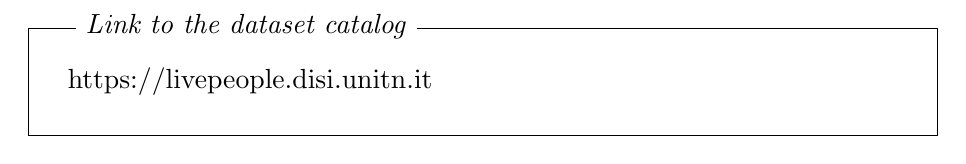
\begin{tikzpicture}[show background rectangle]
\node[align=justify, text width=30em, inner sep=1em]{
\url{https://livepeople.disi.unitn.it}
};
\node[xshift=3ex, yshift=-0.7ex, overlay, fill=white, draw=white, above 
right] at (current bounding box.north west) {
\textit{Link to the dataset catalog}
};
\end{tikzpicture}
\end{center}

\noindent
The catalog simplifies the process of finding and selecting datasets of interest by providing metadata and materials to explore their features. \change{The filter options allow to restrict the search on \dataset data.} It also ensures privacy and copyright compliance, fully respecting the ownership of the authors who contributed to its collection. \change{In addition to the catalog, the webpage available at \url{https://datascientia.disi.unitn.it/projects/diversityone/} collects further information.} The descriptions of downloadable datasets, associated documentation, and procedures for dataset requests are detailed below.

\subsection{Downloadable Datasets and Bundles}

\begin{table}[tb]
    \centering
    \small
    \caption{\change{The size of each bundle of data in Gigabytes, with uncompressed sizes in brackets, and bundle names as they appear in the catalog are presented. Synchronic and diachronic interaction refers to questionnaires and time diaries, respectively.}}\label{tab:sizes}
    \iffalse 
\begin{tabular}{lllllllll}
\toprule
Bundle & \AAU & \AMRITA & \IPICYT & \JLU & \LSE & \NUM & \UC & \UNITN \\
\midrule
App-usage & $<$ 0.1 (0.2) & $<$ 0.1 (0.2) & $<$ 0.1 (0.4) & $<$ 0.1 (0.3) & $<$ 0.1 (0.7) & 0.1 (2.3) & $<$ 0.1 (0.3) & 0.3 (2.8) \\
Connectivity & 0.1 (5.7) & $<$ 0.1 (0.4) & $<$ 0.1 (1.2) & $<$ 0.1 (2.5) & 0.4 (16.8) & $<$ 0.1 (3.7) & $<$ 0.1 (2.8) & 0.6 (26.6) \\
Device-usage & $<$ 0.1 (0.3) & $<$ 0.1 (0.2) & $<$ 0.1 (0.2) & $<$ 0.1 (0.4) & $<$ 0.1 (0.9) & 0.2 (2.3) & $<$ 0.1 (0.4) & 0.5 (4.4) \\
Environment & 0.3 (2.6) & 0.1 (1.4) & 0.6 (6.4) & 0.6 (5.6) & 1.5 (12.1) & 3.3 (35.2) & 0.5 (5.4) & 5.2 (44.5) \\
Motion & 1.9 (18.0) & 1.3 (13.2) & 4.0 (36.8) & 1.2 (12.4) & 7.0 (61.3) & 17.1 (161.3) & 1.8 (19.9) & 18.0 (174.8) \\
Position & 0.6 (5.2) & 0.6 (5.5) & 1.3 (10.2) & 0.1 (1.7) & 2.9 (23.0) & 6.8 (54.7) & 0.8 (7.6) & 12.7 (104.8) \\
Questionnaires & $<$ 0.1  & $<$ 0.1  & $<$ 0.1  & $<$ 0.1  & $<$ 0.1  & $<$ 0.1  & $<$ 0.1  & $<$ 0.1 \\
Time diaries & $<$ 0.1  & $<$ 0.1  & $<$ 0.1  & $<$ 0.1  & $<$ 0.1  & $<$ 0.1  & $<$ 0.1  & $<$ 0.1  \\
\midrule
Total & 2.9 & 2.1 & 6.0 & 2.1 & 12.0 & 27.7 & 3.3 & 37.3 \\
\bottomrule
\end{tabular}
\fi 


\begin{tabular}{lllllllll}
\toprule
\textbf{Bundle name} & \textbf{\JLU} & \textbf{\AAU} & \textbf{\AMRITA} & \textbf{\UNITN} & \textbf{\IPICYT} & \textbf{\NUM} & \textbf{\UC} & \textbf{\LSE} \\
\midrule
App-usage & $<$ 0.1 (0.3) & $<$ 0.1 (0.2) & $<$ 0.1 (0.2) & 0.3 (2.8) & $<$ 0.1 (0.4) & 0.1 (2.3) & $<$ 0.1 (0.3) & $<$ 0.1 (0.7) \\
Connectivity & $<$ 0.1 (2.5) & 0.1 (5.7) & $<$ 0.1 (0.4) & 0.6 (26.6) & $<$ 0.1 (1.2) & $<$ 0.1 (3.7) & $<$ 0.1 (2.8) & 0.4 (16.8) \\
Device-usage & $<$ 0.1 (0.4) & $<$ 0.1 (0.3) & $<$ 0.1 (0.2) & 0.5 (4.4) & $<$ 0.1 (0.2) & 0.2 (2.3) & $<$ 0.1 (0.4) & $<$ 0.1 (0.9) \\
Environment & 0.6 (5.6) & 0.3 (2.6) & 0.1 (1.4) & 5.2 (44.5) & 0.6 (6.4) & 3.3 (35.2) & 0.5 (5.4) & 1.5 (12.1) \\
Motion & 1.2 (12.4) & 1.9 (18.0) & 1.3 (13.2) & 18.0 (174.8) & 4.0 (36.8) & 17.1 (161.3) & 1.8 (19.9) & 7.0 (61.3) \\
Position & 0.1 (1.7) & 0.6 (5.2) & 0.6 (5.5) & 12.7 (104.8) & 1.3 (10.2) & 6.8 (54.7) & 0.8 (7.6) & 2.9 (23.0) \\
Synchronic int. & $<$ 0.1 & $<$ 0.1 & $<$ 0.1 & $<$ 0.1 & $<$ 0.1 & $<$ 0.1 & $<$ 0.1 & $<$ 0.1 \\
Diachronic int. & $<$ 0.1 & $<$ 0.1 & $<$ 0.1 & $<$ 0.1 & $<$ 0.1 & $<$ 0.1 & $<$ 0.1 & $<$ 0.1 \\
\midrule
Total & 2.1 & 2.9 & 2.1 & 37.3 & 6.0 & 27.7 & 3.3 & 12.0 \\
\bottomrule
\end{tabular}

\end{table}

The resources are organized and made available separately considering the full dataset size (approximately 94GB in Parquet format) and GDPR’s minimization principle—which mandates that data must be adequate, limited, and relevant for analysis. Researchers can request access to basic datasets from a specific pilot site (e.g., time diaries collected at \UNITN) or a combination of datasets from multiple pilot sites. To streamline dataset selection, we have created thematic bundles that group data commonly used together for main research purposes. For example, the motion bundle includes all motion sensor data relevant to activity recognition studies, while another bundle, combining questionnaires, time diaries, and location data, is tailored for \cancel{social science research}\change{studying social interactions}. \change{The catalog lists both datasets containing one single sensor and bundles.} \cref{tab:sizes} reports the available bundles (\cref{subsec:ils} details the sensors they contain), and Appendix~\ref{app2:sensors} reports the complete list of sensors in each bundle. \change{Any combination of bundles and single sensors can be downloaded.} All datasets are provided in Parquet format\footnote{Apache Parquet \url{https://parquet.apache.org/}}, an efficient storage format with high compression.
%Larger datasets are divided into manageable chunks to facilitate easier downloading and analysis.
Access to the entire \dataset dataset is also available upon request. 
No source code needs to be made available for the release of this dataset. Future benchmarked datasets derived from our raw dataset will be made available, respecting privacy and copyright, along with code for pre-processing and machine learning-based modeling.

\subsection{Metadata and Documentation}
Each single sensor dataset and bundle is accompanied by metadata and comprehensive documentation that outline content, size, format, and other relevant information.
The catalog user can search the datasets through the metadata values such as the acronym, data collection location, and type of bundle or dataset. The metadata for each dataset and bundle includes:
%
%\begin{enumerate}
    \textit{(i)} A technical report detailing the data collection process;
    \textit{(ii)} Dataset metadata and a codebook with summary statistics;
    \textit{(iii)} Data collection information and links to related projects, including articles published using the dataset;
    \textit{(iv)} Documentation and procedures for dataset requests.
%\end{enumerate}

The catalog enhances the findability, accessibility, and reusability of the dataset in several ways. First, it provides an efficient search method for specific data within a secure institutional environment. Second, it includes concise descriptions that guide users through the available resources, along with detailed information on each dataset, including variable values and labels. Lastly, the technical report and dataset descriptions enable users to analyze the dataset and replicate the data collection process for their own research needs.

\subsection{Dataset Request Process}

\change{We outline the procedure to request the data.
%\begin{enumerate}
First, the user retrieves the identifiers of the bundle or single sensor data of interest from the metadata shown on the catalog for each sensor and bundle.
Second, the metadata also includes a link to the request form, designed together with legal and privacy experts to comply with GDPR and privacy regulations. Interested users affiliated with a research institution can request bundles and datasets by listing the identifiers selected in the previous step and presenting a research proposal. Upon completing the form, users submit their request to the catalog manager using the email address specified in the metadata.} Detailed eligibility criteria and required information are available on the catalog website.
Third, once approved, users must sign a \change{Terms} and License Agreement. Key licensing terms include: \textit{(i)} datasets \cancel{may be}\change{are} used exclusively for research purposes; \textit{(ii)} redistribution of the datasets is prohibited; \textit{(iii)} datasets cannot be publicly shared (e.g., on a website); and \change{\textit{(iv)} any attempt to reverse engineer any portion of the data or to re-identify the participants is strictly forbidden and could constitute unlawful processing of personal data. Finally, the catalog manager sends the instructions for downloading the dataset.}


\section{Discussion} \label{sec:discussion}
 We compared human interpretation data for numerical utterances to LLMs' interpretations, finding substantial differences.
This manifests in LLMs' tendency toward literal interpretations, reversed halo effects (preferring exact interpretations for round rather than sharp numbers; Exp.~1), and inconsistent affect attribution between literal and hyperbolic utterances (Exp.~2), despite human-like prior representations (Exp.~3).
These findings point to a disconnect in LLM pragmatic reasoning --- despite possessing accurate prior knowledge about prices, affect and utterance probabilities --- and despite this knowledge being structured in a way that could support human-like inference when processed through an RSA framework --- LLMs fail to consistently leverage this information when directly prompted to make pragmatic interpretations. 

Our findings highlight an important methodological contribution for understanding LLM behaviors: by systematically decomposing pragmatic reasoning into testable components (priors, affect mappings, utterance likelihoods, and interpretations), we can precisely locate differences between human and AI reasoning. 
This approach extends beyond traditional behavioral comparisons, allowing us to identify whether differences stem from knowledge gaps or reasoning mechanisms. Such detailed cognitive modeling approaches may prove valuable for understanding other aspects of LLM behavior, particularly in cases where surface-level performance masks deeper processing differences from human cognition.
Importantly, our results demonstrate that cognitively-inspired chain-of-thought prompting can help bridge this gap between knowledge and application. We achieved improved correlations with human judgments by decomposing the RSA model's computational steps into natural language reasoning chains. This success suggests that while LLMs may not naturally develop human-like pragmatic reasoning through training alone, they can successfully implement such reasoning when given appropriate computational frameworks that mirror human cognitive processes.

Based on our results, future research could address several important follow-up questions. For instance, potential training modifications to help LLMs better integrate their prior knowledge and context when interpreting hyperbole could be analyzed. Identifying factors that influence how LLMs apply this knowledge in context is also an open question. We report some exploratory analyses (see supplementary materials) that begin to probe these questions through variations in prompting of the models.

Ultimately, our work demonstrates that evaluating LLMs through the lens of cognitive modeling provides a nuanced understanding of how these models deviate from human understanding. By integrating LLMs with cognitive models of pragmatic language use, we can both critically assess the models' internal consistency and provide a framework for improving their performance in interpreting non-literal language.


%\section{Lessons learnt and future work} \label{sec:limits}
%\input{section/06-limits}

\section{Conclusion}\label{sec:conclusion}
\section{Conclusion}\label{sec:conclusion}
This work introduces a novel approach to TOT query elicitation, leveraging LLMs and human participants to move beyond the limitations of CQA-based datasets. Through system rank correlation and linguistic similarity validation, we demonstrate that LLM- and human-elicited queries can effectively support the simulated evaluation of TOT retrieval systems. Our findings highlight the potential for expanding TOT retrieval research into underrepresented domains while ensuring scalability and reproducibility. The released datasets and source code provide a foundation for future research, enabling further advancements in TOT retrieval evaluation and system development.


%\iffalse 
\section{Author contributions}

The names order is by the contribution of the institution and, inside each institution, by the contribution of the individuals. As such, the order of names does not necessarily reflect the importance of the contribution of single individuals. The roles of the authors are presented by their initials as follows:
%
\begin{itemize}
    \item \textit{Study management}: F.G., I.B., A.D.G., M.B.; 
    \item \textit{Study design}: F.G., I.B., G.G., A.D.G., M.B., R.C.A., L.M., D.G.P.; 
    \item \textit{Technical support}: M.R., M.B., R.C.A., L.J.M.;
    \item \textit{Data Collection}: M.B., R.C.A., M.R., A.D.G, P.K., A.G., A.C., G.G., S.S., M.B., L.C., A.H., H.X., D.S., S.D., C.N., S.R.C., A.R.M.;
    \item \textit{Data Preparation and correction}: A.B., R.A.A., I.K., R.C.A., I.B., M.B., D.G.P., L.M.;
    \item \textit{Data analysis}: A.B., L.M.;
    \item \textit{Writing the manuscript}: M.B., A.B., L.M., D.G.P., F.G..
\end{itemize}

%\fi 

%%
%% The acknowledgments section is defined using the "acks" environment
%% (and NOT an unnumbered section). This ensures the proper
%% identification of the section in the article metadata, and the
%% consistent spelling of the heading.

\begin{acks}
    %\grantsponsor{⟨sponsorID⟩}{⟨name⟩}{⟨url⟩}
    %\grantnum[⟨url⟩]{⟨sponsorID⟩}{⟨number⟩}.
    This research has received funding from the \grantsponsor{823783}{European Union's Horizon 2020 FET Proactive} . % leave this dot because there is bug in the macro that delete one character
    project ``WeNet - The Internet of us'', grant agreement No. \grantnum[https://doi.org/10.3030/823783]{823783}{823783}.  We deeply thank all the volunteers across the world for their participation in the study. We thank the anonymous reviewers for their valuable feedback. We acknowledge the use of ChatGPT and Grammarly as tools for grammar refinement.
    \unitn, \jlu, \num and \uc have participated to the work described in this paper as part of the DataScientia initiative (\url{https://datascientia.eu/}).
    %Details regarding funding, including other acknowledgements will be included in a post-double blind review version of the paper. 
\end{acks}

%\begin{acks}
%This research has received funding from the European Union’s Horizon 2020 FET Proactive project “WeNet—The Internet of Us,” grant agreement No 823783. It has deeply benefited from the many discussions that we have had with all the people working in the WeNet project.
%\end{acks}

%%
%% The next two lines define the bibliography style to be used, and
%% the bibliography file.
\bibliographystyle{ACM-Reference-Format}
\bibliography{main}


%%
%% If your work has an appendix, this is the place to put it.
\newpage
\appendix

\section{APPENDIX}

\section{How is MENTAT Different from Medical Exam Questions?}
\label{app:medqa_to_mentat}

For years, medical AI benchmarks have focused on fact-based assessments. Most medical evaluations for LMs rely on board exams and medical student tests, primarily measuring knowledge recall rather than real-world clinical decision-making. These exams have little correlation with actual clinical practice, as passing them does not equate to the ability to manage patients effectively even in humans \cite{Saguil2015}.

\begin{figure}[ht]
    \begin{framed}
    A 32-year-old woman with type 1 diabetes mellitus has had progressive renal failure during the past 2 years. 
    She has not yet started dialysis. Examination shows no abnormalities. Her hemoglobin concentration is 9 g/dL, 
    hematocrit is 28\%, and mean corpuscular volume is 94 $\mu$m\textsuperscript{3}. 
    A blood smear shows normochromic, normocytic cells. 
    Which of the following is the most likely cause?
    
    (A) Acute blood loss \\
    (B) Chronic lymphocytic leukemia\\
    (C) Erythrocyte enzyme deficiency\\
    (D) Erythropoietin deficiency\\
    (E) Immunohemolysis\\
    (F) Microangiopathic hemolysis\\
    (G) Polycythemia vera \\
    (H) Sickle cell disease \\
    (I) Sideroblastic anemia \\
    (J) $\beta$-Thalassemia trait\\
    \textbf{(Answer: D)}
    \end{framed}
    \caption{USMLE board exam question example }
    \label{fig:usmle_example_q}
\end{figure}




For example, \Cref{fig:usmle_example_q} presents a classic USMLE board exam question \cite{USMLE2021}, which tests an AI model’s ability to recall factual knowledge rather than apply practical decision-making skills. The question may assess the recognition of a laboratory abnormality in diabetes, but it does not evaluate whether the model can adjust insulin regimens, recognize psychosocial factors, or determine hospitalization needs—key components of real-world patient care. As highlighted in previous research, medical licensing exams do not strongly correlate with clinical competency, reinforcing the need for benchmarks that evaluate accurate decision-making skills rather than memorization.

\begin{table}[h]
    \centering
    \begin{tabular}{llp{10cm}}
        \toprule
        \textbf{Question type} & \textbf{Attribute type} & \textbf{Example template question} \\
        \midrule
        \multirow{6}{*}{Single-Verify} 
        & SCP Code & Does this ECG show symptoms of \textbf{non-specific ST changes}? \\
        & Noise & Does this ECG show \textbf{baseline drift in lead I}? \\
        & Stage of infarction & Does this ECG show \textbf{early stage of myocardial infarction}? \\
        & Extra systole & Does this ECG show \textbf{ventricular extrasystoles}? \\
        & Heart axis & Does this ECG show \textbf{left axis deviation}? \\
        & Numeric feature & Does the \textbf{RR interval} of this ECG fall \textbf{within the normal range}? \\
        \bottomrule
    \end{tabular}
    \caption{Example template questions for different ECG attributes.}
    \label{tab:ecg_questions}
\end{table}
\begin{table}[h]
    \centering
    \begin{tabular}{lp{3.cm}p{3.5cm}p{1.5cm}p{3.5cm}}
        \toprule
        \textbf{Category} & \textbf{Task} & \textbf{Prompt} & \textbf{Result} & \textbf{AI Response} \\
        \midrule
        \multirow{2}{*}{Sequence alignment} 
        & DNA sequence alignment to human genome 
        & Align the DNA sequence to the human genome: \texttt{TGGGCTCA AGTGATCATA……} 
        & chr7 
        & As a language model AI, I do not have the capability to align a DNA sequence to the human genome…… 
        \\
        \midrule
        & DNA sequence alignment to multiple species 
        & Which organism does the DNA sequence come from: \texttt{CGTACACC ATTGGTGC……} 
        & yeast 
        & The organism from which the DNA sequence comes cannot be determined based solely on the DNA sequence…… 
         \\
        \bottomrule
    \end{tabular}
    \caption{DNA Sequence Alignment Tasks and AI Responses}
    \label{tab:sequence_alignment}
\end{table}


\Cref{tab:ecg_questions} and \Cref{tab:sequence_alignment} illustrate additional examples of widely used AI benchmarks, such as ECG-QA \cite{Oh2024} and GeneTuring \cite{Hou2023}, which focus on highly structured, fact-based medical knowledge. These datasets and others like MedQA \cite{Jin2021} have been leveraged by major AI companies, including Google’s Gemini initiative \cite{Saab2024}, to highlight model performance. While these benchmarks evaluate text-based and multimodal AI capabilities, they focus heavily on fact memorization rather than applied clinical reasoning.

Unlike traditional medical AI benchmarks, MENTAT is designed by practicing psychiatrists to reflect real-world clinical scenarios. The dataset also includes ambiguous, multi-choice decision-making tasks rather than a single correct answer, simulating the complex nature of psychiatric practice. Furthermore, MENTAT aims to reduce bias by empowering a diverse group of clinicians in its development from the start, making it less likely to reinforce harmful racial, gender, or sexuality-based biases in mental healthcare. In summary, MENTAT differs from medical exam questions by moving beyond fact recall to assess practical clinical decision-making in mental healthcare. While traditional benchmarks test AI models on medical knowledge, MENTAT evaluates whether AI can handle real-world psychiatric tasks, manage patient uncertainty, and make informed decisions in complex clinical environments.




% For years, benchmark evaluations have been utilized in medical AI to track the progress of new and updated models. However, they have largely focused on genetics, radiology, cardiology, and electronic medical record data processing\cite{Hou2023, Zambrano2023, Oh2024}. Little work has thus far been invested in the creation of benchmark evaluations and datasets for mental healthcare. Most medical evaluations of language and multi-modal models have also only focused on specialty board exams and exams intended for medical students. Both categories of exams assess knowledge but have been noted to have relatively little correlation to the real-world practice of medicine\cite{Saguil2015}. Every medical specialty would benefit from a creation of a dataset of question-answer pairs tailored specifically to clinical practice as opposed to the fact-based assessment that is common in licensing and medical student exams. As an example, Figure 1 demonstrates a classic board exam question directly from the USMLE website \cite{USMLE2021}, a medical licensing exam all medical students must take. It does not assess knowledge about pragmatic clinical management of diabetes; rather, it focuses on fact-based knowledge. Just as Saguil et al highlighted a lack of correlation between medical licensing exams and clinical skills, a model’s ability to answer Figure 1 correctly does not correlate to its ability to care for an individual with diabetes. Construction of datasets that test practical medical knowledge are necessary to robustly evaluate language models’ appropriateness in clinical settings. Furthermore, clinicians have recently called for moving beyond a medical exam benchmark, stating, "it is essential to move beyond medical exams and adopt more grounded, task-specific approaches for evaluation" \cite{Raji2025}. A related study, published in 2025, identified 11 high-level clinical tasks and created a benchmark (MedS-bench) meant to "address this gap" as current benchmarks and evaluation datasets "fail to adequately reflect the practical utility of LLMs in real-world clinical scenarios". Our work is different, but complementary, as our dataset applies this concept (testing for skills required to practice as a clinician as opposed to esoteric medical facts) to mental healthcare. In the realm of mental healthcare, researchers have expanded evaluations of LLM's into the realm of psychotherapy, which is complementary to our approach of evaluating LLM performance in the related field of psychiatry.


% As previously mentioned, most investigations into the evaluation of AI models in the healthcare setting have focused on pre-existing fact-based datasets such as the USMLE exams and specialty-specific board exams. In practice, these knowledge-based tests (e.g., USMLE Step 1) are designed to assess whether human trainees have acquired sufficient baseline knowledge to enter post-graduate training in a selected medical specialty. However, passing these tests alone is not considered sufficient for practicing as a physician in the United States. Residency training is required, during which trainees apply fundamental medical knowledge to real-world clinical cases \cite{Mowery2015}. 
% %
% Similarly, AI models must progress beyond simple recall of medical facts. They should be trained and evaluated on real-world clinical tasks that require the application of baseline medical knowledge. To maximize external validity, datasets should be created and vetted by actively practicing clinicians. Some of the most widely used benchmarks in medical AI are frequently leveraged by major companies to showcase the clinical capabilities of their fine-tuned models. For instance, in 2024, Google published *Capabilities of Gemini Models in Medicine*, incorporating several prominent medical benchmarks \cite{Saab2024}. The authors highlight the novelty of their work as “the most comprehensive benchmarking of multimodal medical models to date” based on their use of 14 different medical benchmarks \cite{Saab2024}. These benchmarks include ECG-QA \cite{Oh2024}, MedQA \cite{Jin2021}, GeneTuring \cite{Hou2023}, MMMU (health medicine) \cite{Yue2023}, NEJM Image Challenges \cite{NEJM2024}, Path-VQA \cite{He2020}, and others. Additionally, an effort was made to enhance the clinical relevance of these findings by evaluating the models’ ability to summarize complex medical information and generate referral letters for specialists \cite{Saab2024}. 
% %
% Examples of questions from these datasets are provided in Figures 3 and 4, which illustrate excerpts from ECG-QA and GeneTuring, respectively. MedQA, on the other hand, is best represented by the example in Figure 1. In the domain of mental health datasets and summarization, Adhikary et al. introduced a dataset comprising 191 counseling sessions with associated summaries \cite{Adhikary2024}. 
% %
% Despite the breadth of existing benchmarks, there is still no robust, clinician-led, and clinician-vetted mental healthcare benchmark for AI models. Current medical benchmarks remain overly narrow and fact-based, limiting their external validity and clinical relevance. As noted earlier, a high score on the MedQA benchmark does not equate to excellence in clinical care. Our dataset shifts the paradigm by moving beyond fact-based assessments (e.g., USMLE exams) and introducing a comprehensive evaluation of clinician-level decision-making in mental healthcare. 
% %
% Our benchmark uniquely assesses an AI model’s ability to **triage, diagnose, treat, and monitor mental health conditions**, establishing a new category of medical benchmarks that we hope other specialties will adopt. Furthermore, because our dataset is developed and overseen by a diverse group of practicing clinicians, it is significantly less likely to perpetuate harmful racial, gender, or sexuality-based biases in mental healthcare. It has been validated by [insert number] practicing psychiatrists.

\newpage

\section{Further Annotation Processing Results}
\label{app:annotation_details}

% \begin{figure}[ht]
%     \vskip 0.2in
%     \begin{center}
%     \centerline{\includegraphics[width=0.5\columnwidth]{figures/raw_annotation_krippendorf.pdf}}
%     \caption{Test.}
%     \label{fig:raw_annotation_krippendorf}
%     \end{center}
%     \vskip -0.2in
% \end{figure}

\begin{figure}[ht!]
    \centering
    \begin{minipage}[b]{0.49\textwidth}
        \centering
        \includegraphics[width=\linewidth]{figures/annotator_scores_hbt_pars.pdf}
        \caption{(Top) We show the average raw annotation score with with bootstrapped (95\% CL) uncertainties for each annotator. All of them deviate from 50 with statistical significance (the random baseline). 
        (Bottom) Fitted individual annotator parameters from the hierarchical Bradley-Terry model.
        Besides regularization in the log-likelihood objective, we bound the individual annotator parameters ($\gamma_a \in [-3.0, 3.0]$, $\alpha_a \in [0.5, 2.0]$) during the optimization to balance the goal of slightly de-noising the resulting preference dataset while keeping the majority of differences between individual annotator preferences.
        These bounds prevent the model from fixing contradictory data by pushing a parameter to an extreme.
        The fact that all annotators have a positive offset $\gamma_a$ indicates that they all tend to choose one answer option to prefer over all others in a single annotation of one question.}
        \label{fig:annotator_scores_hbt_pars}
    \end{minipage}%
    \hfill
    \begin{minipage}[b]{0.49\textwidth}
        \centering
        \includegraphics[width=\linewidth]{figures/raw_annotation_krippendorf.pdf}
        \caption{
        We show the distribution of  Krippendorff's $\alpha$ for raw triage and documentation question annotations.
        We verify that the expert annotators do not converge on one answer option and that there is sufficient inter-annotator disagreement.
        Given our design choices, we expect $\alpha$ to be naturally low as our goal is not to measure the presence of a single ground truth and low $\alpha$ values ($\alpha \leq 0.5$) will not tell us how useful a set of annotations is—only that experts statistically disagree. 
        }
        \label{fig:raw_annotation_krippendorf}
    \end{minipage}
\end{figure}
% \begin{figure}[ht]
%     \vskip 0.2in
%     \begin{center}
%     \centerline{\includegraphics[width=0.5\columnwidth]{figures/annotator_scores_hbt_pars.pdf}}
%     \caption{Test.}
%     \label{fig:annotator_scores_hbt_pars}
%     \end{center}
%     \vskip -0.2in
% \end{figure}
% \begin{figure}[ht]
%     \vskip 0.2in
%     \begin{center}
%     \centerline{\includegraphics[width=0.5\columnwidth]{figures/frac_ct in topk_bt_vs_hbt.pdf}}
%     \caption{Test.}
%     \label{fig:frac_ct in topk_bt_vs_hbt}
%     \end{center}
%     \vskip -0.2in
% \end{figure}

\newpage

\section{Language Model Prompts}
\label{app:prompting}

\begin{figure}[ht]
    \centering
    \begin{minipage}[b]{0.38\textwidth}
        \begin{framed}
        \texttt{
        f"Question: \{q\}\textbackslash n\textbackslash n"\\
        f"A: \{answer\_list[0]\}\textbackslash n"\\
        f"B: \{answer\_list[1]\}\textbackslash n"\\
        f"C: \{answer\_list[2]\}\textbackslash n"\\
        f"D: \{answer\_list[3]\}\textbackslash n"\\
        f"E: \{answer\_list[4]\}\textbackslash n\textbackslash n"\\
        "Answer (single letter): "
        }
        \end{framed}
    \end{minipage}%
    \hfill
    \begin{minipage}[b]{0.62\textwidth}
        % \centering
        \begin{framed}
        \texttt{
        f"Question: \{q\}\textbackslash n\textbackslash n"\\
        f"A: \{answer\_list[0]\}\textbackslash n"\\
        f"B: \{answer\_list[1]\}\textbackslash n"\\
        f"C: \{answer\_list[2]\}\textbackslash n"\\
        f"D: \{answer\_list[3]\}\textbackslash n"\\
        f"E: \{answer\_list[4]\}\textbackslash n\textbackslash n"\\
        "Answer (only reply with a single letter!): "
        }
        \end{framed}
    \end{minipage}
    \caption{(Left) Prompt text MCQA variation A (as used for \textit{gpt-4o-mini-2024-07-18}, \textit{gpt-4o-2024-08-06}, \textit{o1-2024-12-17}, and \textit{o1-mini-2024-09-12}).
    (Right) Prompt text MCQA variation B (all other models).
By looking at the responses from models evaluated with variation A, we verified that the recorded accuracy difference caused by using different promtps was $\leq 1$\%.
The only exception was \textit{o1-mini-2024-09-12}, for which we corrected the evaluation.}
    \label{fig:eval_prompts_mcqa}
\end{figure}

\begin{figure}[ht]
    \vskip 0.2in
    \begin{framed}
        \texttt{
        f"Question: \{q\}\textbackslash n\textbackslash n"\\
        "Answer (write your reply in only one short sentence!): "
        }
        \end{framed}
        \caption{Prompt text free-form (as used for the models evaluated in \Cref{sec:4_4_consistency}).}
    \vskip -0.2in
\end{figure}

\newpage

\section{Annotator Interface}
\label{app:annotator_interface}

\begin{figure}[ht]
    \centering
    \begin{minipage}[b]{0.49\textwidth}
        \centering
        \includegraphics[width=\linewidth]{figures/mentat_q36_question.png}
    \end{minipage}%
    \hfill
    \begin{minipage}[b]{0.49\textwidth}
        \centering
        \includegraphics[width=\linewidth]{figures/mentat_q36_answers.png}
    \end{minipage}
    \caption{Example of the online annotation interface using the \textit{jsPsych} library \citep{de_Leeuw2023} (MIT license). There is also a comment box below the sliders for feedback/comments, that is not shown.}
    \label{fig:mentat_q36_combined}
\end{figure}

\newpage

\section{Further Evaluation Results}
\label{app:more_experiment_results}

\begin{figure}[ht]
    \centering
    \begin{minipage}[b]{0.49\textwidth}
        \centering
        \includegraphics[width=\linewidth]{figures/final_eval_results_by_gender.pdf}
        \caption{Using the $\mathcal{D}_\text{G}$ dataset, we evaluate eleven off-the-shelf instruction-tuned and three (mental) healthcare fine-tuned models for overall accuracy and how it is impacted by different patient genders.}
        \label{fig:final_eval_results_by_gender}
    \end{minipage}%
    \hfill
    \begin{minipage}[b]{0.49\textwidth}
        \centering
        \includegraphics[width=\linewidth]{figures/final_eval_results_by_age.pdf}
        \caption{Using the $\mathcal{D}_\text{A}$ dataset, we evaluate eleven off-the-shelf instruction-tuned and three (mental) healthcare fine-tuned models for overall accuracy and how it is impacted by different patient ages.}
        \label{fig:final_eval_results_by_age}
    \end{minipage}
\end{figure}

% \begin{figure}[ht]
%     \vskip 0.2in
%     \begin{center}
%     \centerline{\includegraphics[width=0.5\columnwidth]{figures/final_eval_results_by_gender.pdf}}
%     \caption{Test.}
%     \label{fig:final_eval_results_by_gender}
%     \end{center}
%     \vskip -0.2in
% \end{figure}
% \begin{figure}[ht]
%     \vskip 0.2in
%     \begin{center}
%     \centerline{\includegraphics[width=0.5\columnwidth]{figures/final_eval_results_by_age.pdf}}
%     \caption{Test.}
%     \label{fig:final_eval_results_by_age}
%     \end{center}
%     \vskip -0.2in
% \end{figure}

\begin{figure}[ht!]
    \vskip 0.2in
    \begin{center}
    \centerline{\includegraphics[width=0.47\columnwidth]{figures/final_eval_results_by_nat.pdf}}
    \caption{Using the $\mathcal{D}_\text{N}$ dataset, we evaluate eleven off-the-shelf instruction-tuned and three (mental) healthcare fine-tuned models for overall accuracy and how it is impacted by different patient ethnicities.}
    \label{fig:final_eval_results_by_nat}
    \end{center}
    \vskip -0.2in
\end{figure}


\end{document}
\endinput
%%
%% End of file `sample-manuscript.tex'.
